\chapter{Physics Building Blocks and their Reconstruction}
\label{chap:objects}

\epigraph{\textit{If you can put your five fingers through it it is a gate, if not a door.}}{--Stephen Dedalus, in James Joyce's \textit{Ulysses}}

In order to convert the multitude of electrical signals read out by the subdetectors
of ATLAS as a result of a sucessful trigger (c.f. Section~\ref{sec:tdaq})
into well-defined and meaningful representations of the underlying physics process
that initiated them, at the level required for performing high-quality physics analysis,
several steps of reconstruction and identification must take place.
The physics analyses presented in the current work involve the use of leptons,
jets, and the so-called missing transverse momentum, \ptmiss.
The methods used to deduce the presence of these objects within the ATLAS detector
will be discussed in this chapter.
Section~\ref{sec:tracks_and_vertices} introduces the reconstruction of charged-particle
tracks and $pp$ interaction vertices within the ID, both of which are used as low-level seeds or inputs to the
reconstruction of the high-level physics objects to be discussed in the subsequent
sections.
Section~\ref{sec:leptons} goes on to discuss the reconstruction of the charged leptons
relevant to the current work: electrons and muons.
Sections~\ref{sec:jets} and \ref{sec:flavor_tagging} describe the reconstruction
of jet objects and the identification of jets arising from the decay of heavy-flavor hadrons,
respectively.
Section~\ref{sec:met} then goes on to describe the reconstruction of \ptmiss,
which relies on an accurate description of leptons and jets.
The methods used for reconstructing the leptons and jets are not one hundred percent
accurate: detector information arising due to an electron may leave signatures
similar to those of a jet, for example, and thus spoil their unambiguous description.
Where relevant, in the following we will discuss the methods by which the reconstruction
and identification of the physics objects is made more precise and how high levels
of confidence about their actual presence within the detector are achieved.
Section~\ref{sec:object_ambiguity} will also introduce the notion of high-level
object ambiguity resolution through the use of so-called \textit{overlap removal}
procedures.

%%%%%%%%%%%%%%%%%%%%%%%%%%%%%%%%%%%%%%%%%%%%%%%%%%%%%%%%%%%%%%%%%%%
%%%%%%%%%%%%%%%%%%%%%%%%%%%%%%%%%%%%%%%%%%%%%%%%%%%%%%%%%%%%%%%%%%%
%% TRACKING AND VERTEXING
%%%%%%%%%%%%%%%%%%%%%%%%%%%%%%%%%%%%%%%%%%%%%%%%%%%%%%%%%%%%%%%%%%%
%%%%%%%%%%%%%%%%%%%%%%%%%%%%%%%%%%%%%%%%%%%%%%%%%%%%%%%%%%%%%%%%%%%
\section{Charged-Particle Tracks and Primary Vertices}
\label{sec:tracks_and_vertices}

The reconstruction of charged-particle tracks (`tracking') and primary interaction
vertices (`vertexing') is based on information provided by the ID, primarily by the
the pixel and SCT subdetectors~\cite{NEWTracking,TIDE,Aaboud:2016rmg,ATLAS-CONF-2010-069,Piacquadio_2008}.
Charged-particles produced in $pp$ collisions will leave signals --- \textit{hits} ---
on the different layers of the ID.
The aim of tracking is to translate these layer hits into \textit{spacepoints}
which are then combined to form a track following the particle's traversal trough the ID.
Given its highly granular readout, the pixel detector provides three dimensional spacepoints
from each layer hit while the back-to-back readout strips on each layer of the SCT 
must be combined, using the stereo-angle information from the second set of strips, to
give three dimensional spacepoint information.
The hit information provided by the TRT straws is two-dimensional in nature, providing only
$r-\phi$ information in the barrel section and $\phi-z$ information in the end-caps.

Within the solenoidal magnetic field of the ID, charged-particle tracks follow
helical trajectories in the plane transverse to the beam-pipe ($xy$-plane) and
can be fully characterised by five \textit{track (perigee) parameters}:
\begin{align}
    \left(d_0, z_0, \phi, \theta, q/p\right),
    \label{eq:track_parameters}
\end{align}
where $d_0$ ($z_0$) is the transverse (longitudinal) impact parameter,
$\phi$ and $\theta$ are the azimuthal and polar coordinate, respectively, of the track at the
point at which $d_0$ and $z_0$ are defined, $q/p$ is the ratio of the particle charge
to the magnitude of its momentum.
The charge of a track is determined by its curvature within the magnetic field.
The track parameters are defined with respect to their associated primary
vertex, whose reconstruction will be described shortly.
An illustration describing the track parameters is provided by Figure~\ref{fig:track_params}.

The primary track reconstruction algorithm used in ATLAS follows an \textit{inside-out} pattern
recognition procedure and first starts with information
provided by track \textit{seeds}, composed of a few spacepoints, in the silicon detectors
which then are extended outwards into the TRT~\cite{NEWTracking}.
The inside-out approach accounts for the majority of tracks reconstructed in ATLAS but
it is complemented by an \textit{outside-in} approach that starts with the TRT hits and moves
inwards~\cite{NEWTracking}.
This latter approach is useful in recovering those tracks with ambiguous or missing inner-layer pixel hits;
for example, in the case of photon
conversions or long-lived neutral particle decays.

The collection of reconstructed tracks is used as input to the primary vertex reconstruction.
%A properly reconstructed primary vertex, from which a set of charged-particle tracks originate,
%indicates the likely position of a hard $pp$ interaction and around which subsequent event reconstruction
%will take place~\cite{Aaboud:2016rmg,Piacquadio_2008}.
Primary vertex reconstruction follows a so-called \textit{adaptive vertex fitting} (AVF)~\cite{Aaboud:2016rmg,Piacquadio_2008}
procedure and occurs in two steps: primary vertex finding,
in which tracks are associated to a particular vertex candidate, and vertex fitting,
which involves the reconstruction of the actual vertex position and its errors.
After the vertex fitting stage, the tracks associated with a given vertex are refit
with the constraint of the vertex position and its errors. The track refitting can update
the track parameters (Eqn.~\ref{eq:track_parameters}) associated with the tracks.
Only vertices with at least two charged particle tracks with $\pT > 400\,\MeV$ are
considered.

In the high luminosity collisions at the LHC there will generally be multiple primary vertices
associated with each $pp$ bunch crossing.
A physics \textit{event} in ATLAS, then, is chosen as the set of processes originating from the $pp$ interaction
associated with the \textit{hardest} primary vertex --- the \textit{primary hard-scatter vertex} --- taken as that primary vertex with the
highest sum of squared \pT~of tracks originating from that vertex.
The subsequent event reconstruction takes place around the primary hard-scatter vertex and only
those objects originating from it are taken as relevant when reconstructing the physics objects in the event.
Any additional primary vertices are considered as \textit{pileup vertices}.

The presence of so-called \textit{secondary}, \textit{tertiary}, and so on..., vertices are also
important and will be described in Section~\ref{sec:flavor_tagging}.

\begin{figure}[!htb]
    \begin{center}
        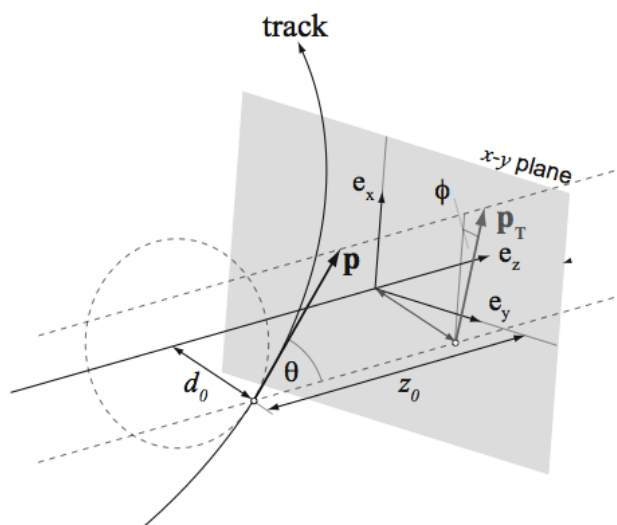
\includegraphics[width=0.6\textwidth]{figures/chapter3/perigee_params}
        \caption{
            Illustration of the relationship between the track parameters and associated track.
            In this scenario, the hard scatter primary vertex is located
            at $(e_x, e_y, e_z) = (0,0,0)$, though this is not generally the case.
        }
        \label{fig:track_params}
    \end{center}
\end{figure}

\begin{figure}[!htb]
    \begin{center}
        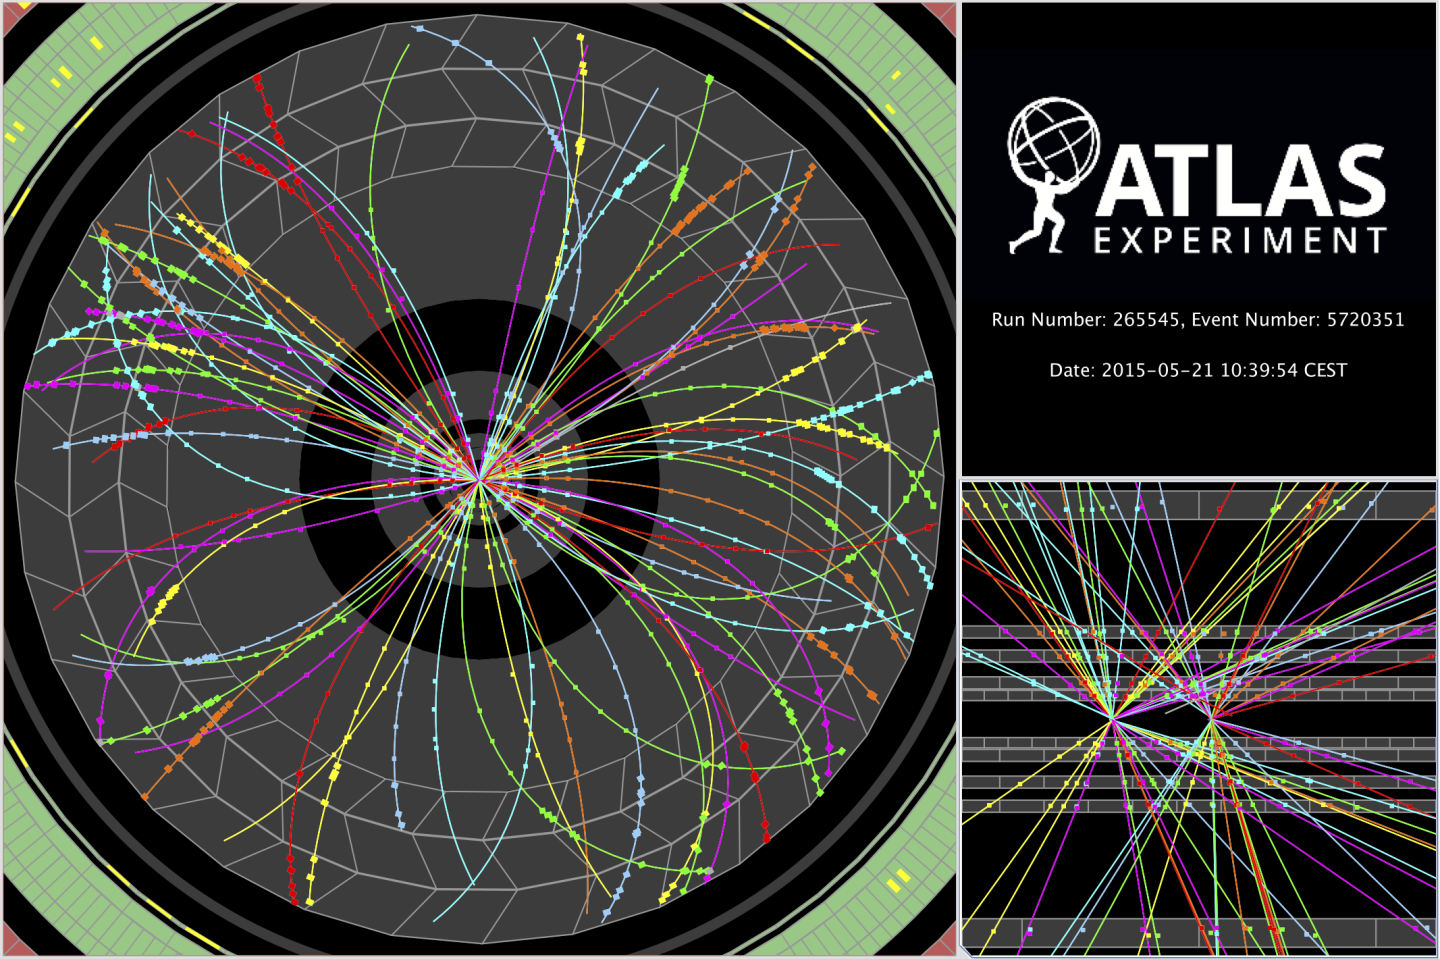
\includegraphics[width=0.7\textwidth]{figures/chapter3/event_display_tracking_vertexing}
        \caption{
            Event display of a low-pileup event recorded at the start of Run-II, in early 2015.
            \textit{Left}: Transverse view of the ID. Seen in color are the reconstructed tracks traversing
                the inner layers of the pixel detector, SCT, and TRT. The colored dots are all reconstructed
                spacepoints used as input to the track fitting procedure.
            \textit{Right,\,lower}: View in $r-z$ of the same $pp$ bunch-crossing event as on the left.
                Two reconstructed primary vertices are clearly observed.
                On average, in Run-II there were roughly 30 primary vertices reconstructed per event, with
                up to $\approx65$ occuring at maximum.
        }
        \label{fig:id_event_display}
    \end{center}
\end{figure}
\FloatBarrier


%%%%%%%%%%%%%%%%%%%%%%%%%%%%%%%%%%%%%%%%%%%%%%%%%%%%%%%%%%%%%%%%%%%
%%%%%%%%%%%%%%%%%%%%%%%%%%%%%%%%%%%%%%%%%%%%%%%%%%%%%%%%%%%%%%%%%%%
% LEPTONS
%%%%%%%%%%%%%%%%%%%%%%%%%%%%%%%%%%%%%%%%%%%%%%%%%%%%%%%%%%%%%%%%%%%
%%%%%%%%%%%%%%%%%%%%%%%%%%%%%%%%%%%%%%%%%%%%%%%%%%%%%%%%%%%%%%%%%%%
\section{Electrons and Muons}
\label{sec:leptons}

Electrons and muons, being charged particles, leave identifiable tracks
within the ID.
As a result, their reconstruction involves the use of the tracks and
vertices described in the previous section, using them essentially as initial
seeds for their complete reconstruction.
Electron reconstruction, described in Section~\ref{sec:electrons}, complements the track information provided by the ID
with calorimetric information provided by the EM calorimeter (Section~\ref{sec:calo_em})
and with knowledge about the pattern of transition radiation expected to occur
in the TRT as a result of passing electrons.
Muon reconstruction, described in Section~\ref{sec:muons}, revolves around stitching together the tracks reconstructed
in the ID with those tracks independently reconstructed in the MS layers at large radii.

\subsection{Electrons}
\label{sec:electrons}

\subsubsection{Electron Reconstruction}
\label{sec:electron_reco}

{\color{red}{After 2016 they replaced sliding window algorithm with supercluster-based reco}}

The reconstruction of electron candidates is based on three components which
characterise the signature of electrons: localised clusters of energy
deposits found within the EM calorimeter, charged-particle tracks
identified in the ID, close-matching (in ($\eta,\phi$)) of the tracks to the clusters
that form the final electron candidates~\cite{Aad:2019tso}.
It is generally possible to match multiple tracks to the same electrogmagnetic cluster,
all originating from the same primary electron produced in the hard-scatter.
This is due to the fact that electrons lose significant amounts of energy to bremsstrahlung
photons as they interact with and traverse the ID.
These radiated photons can then undergo conversion to electron-positron pairs,
which, too, can undergo further bremsstrahlung.
The positrons, electrons, and photons are usually emitted in a very collimated fashion
and thus deposit most of their energy in a localised fashion within the calorimter.

The search for localised energy deposits in the EM calorimeter is performed
by following a sliding window algorithm over the individual cells whose dimensions are
defined by the second sampling layer of the EM calorimeter (Figure~\ref{fig:em_calo_section}).
Electron candidates are seeded by localised energy deposits whose summed transverse energy,
across all layers of the EM calorimeter, is greater than $2.5\,\GeV$~\cite{Aad:2019tso}.
These clusters act as seeds for the matching of reconstructed ID tracks.
The reconstructed tracks are refit using a Gaussian Sum Filter (GSF) method~\cite{ATLAS-CONF-2012-047} 
that accurately accounts for the bremsstrahlung energy losses characteristic of
electron traversal and are then matched to the localised clusters using
the cluster barycenter as the point of reference to match in $\eta-\phi$.
If there is no GSF-track candidate matching to the EM calorimeter cluster seed, then
the cluster is marked as an unconverted photon. The cluster is marked as a
converted photon if a matched GSF-track candidate exists but is not associated
with the primary hard-scatter vertex.

\subsubsection{Electron Identification}
\label{sec:electron_id}

Once electron candidates are reconstructed, they are selected based on various
levels of identification.
A further set of identification criteria is required on top of the reconstruction
so as to improve the selection of true electrons originating from the primary hard-scatter
vertex --- so-called \textit{prompt} electrons --- over \textit{non-prompt} sources
of reconstructed electrons such as those originating from photon conversions or the misidentifiation
of charged pions that leave electron-like tracks in the ID.
This identification criteria is based on the construction of a multivariate likelihood (LH) and
is referred to as the \textit{electron likelihood identification}.
The inputs to the LH are listed in Table~\ref{tab:egamma_lh_inputs} and include measurements from the tracking system in the ID,
calorimetric information, and quantities that combine the tracking and calorimetric information~\cite{Aad:2019tso}.

\begin{figure}[!htb]
    \begin{center}
        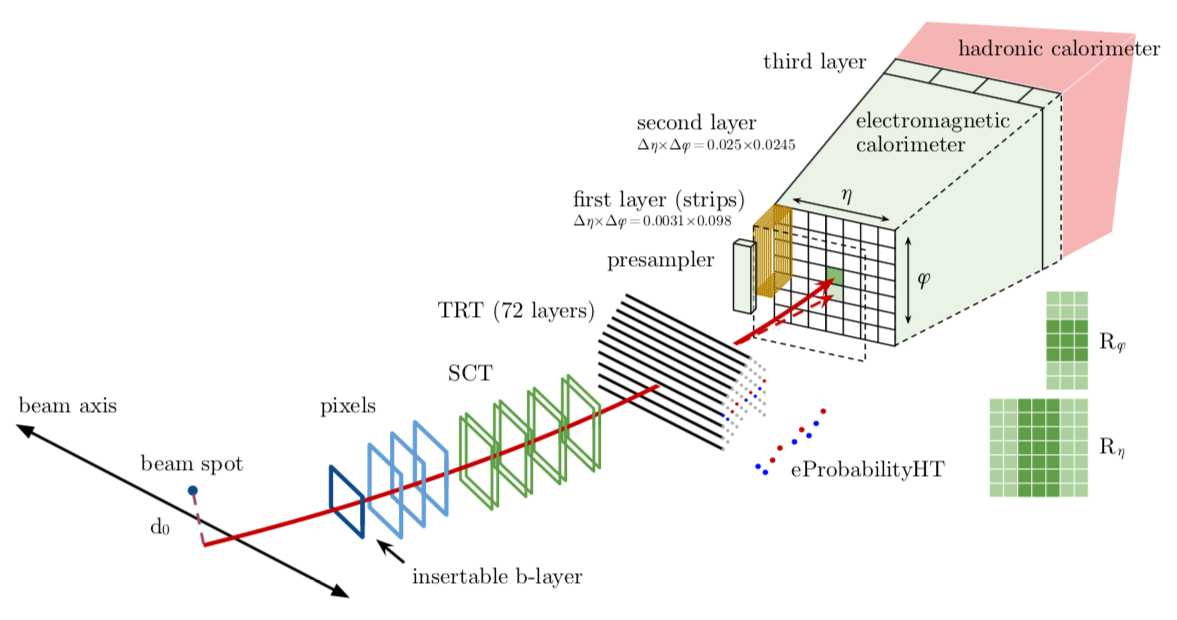
\includegraphics[width=0.9\textwidth]{figures/chapter3/egamma/egamma_lh_input_desc}
        \caption{
        }
        \label{fig:egamma_lh_input_desc}
    \end{center}
\end{figure}

The electron LH is based on the products for the signal and background probability density
functions (PDFs) associated with the set of inputs in Table~\ref{tab:egamma_lh_inputs}:

\begin{align}
    L_{S\,(B)}(\mathbf{x}) = \prod\limits_{i=1}^n P_{S\,(B),i} (x_i),
    \label{eq:egamma_lh}
\end{align}
where $\mathbf{x}$ is the vector of quantities listed in Table~\ref{tab:egamma_lh_inputs} and
the $P_{S\,(B),i}(x_i)$ are the values of the PDF for quantity $i$ at value $x_i$ for the
signal ($S$) and background ($B$).
The likelihoods are built using simulation and the signal is composed of samples of prompt electrons
and the background is built from a combination of jets that mimic the signature of
prompt electrons, electrons from photon conversions, and non-prompt electrons from the decay
of hadrons containing heavy-flavours~\cite{Aad:2019tso}.
The final electron LH discriminant, shown in Figure~\ref{fig:egamma_lh_discriminant}, is based on a transformed version of the ratio,
\begin{align}
    d_L = \frac{L_S}{L_S + L_B},
    \label{eq:egamma_lh_disc}
\end{align}
where the transformation acts to spread $d_L$ to values not bounded by $0$ and $1$,
motivated by the need to have well-defined working points based on selections on $d_L$.

There are four such fixed values of the final LH discriminant that are used to define
four working points corresponding to increasing thresholds on the final LH discriminant:
\textsc{VeryLoose}, \textsc{Loose}, \textsc{Medium}, and \textsc{Tight}.
The efficiencies to identifiy prompt electron candidates are measured using samples of $Z\rightarrow ee$ and
$J/\psi \rightarrow ee$ following a tag-and-probe approach.
They are found, for electron candidates with $E_T > 40\,\GeV$,
to be 93\%, 88\%, and 80\% for the \textsc{Loose}, \textsc{Medium}, and \textsc{Tight} working points, respectively~\cite{Aad:2019tso}.

\begin{figure}[!htb]
    \begin{center}
    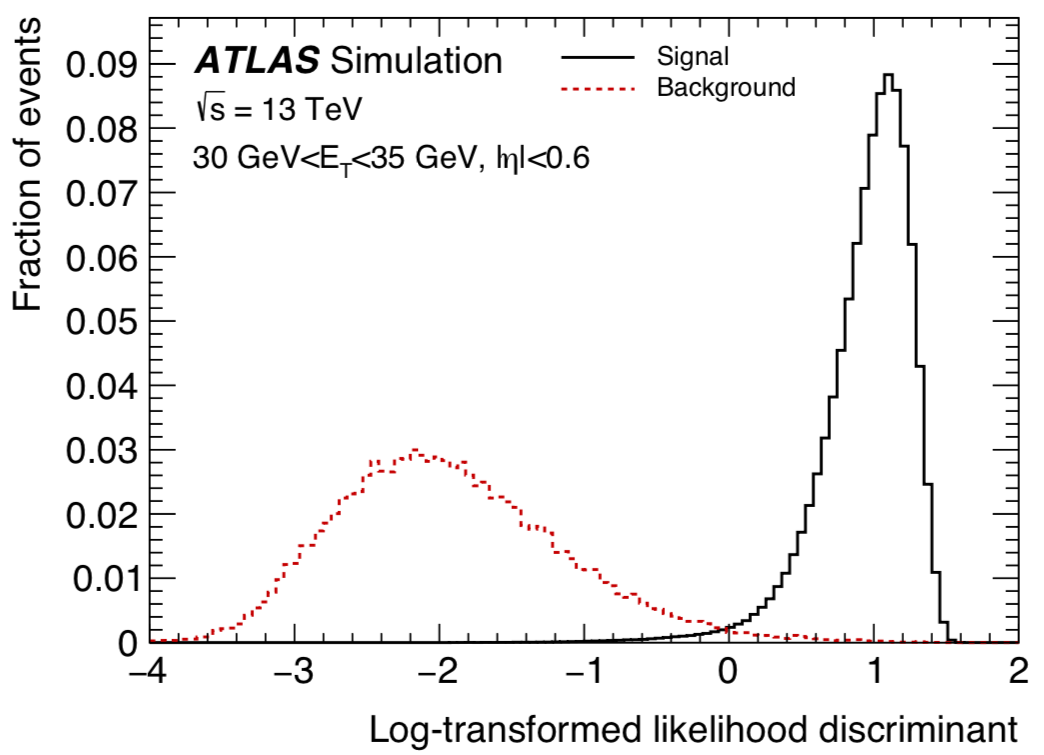
\includegraphics[width=0.7\textwidth]{figures/chapter3/egamma/egamma_lh_discriminant}
    \caption{
        Transformed LH-based electron identification discrimiant for electron candidates
        with $30\,\GeV < E_T < 35\,\GeV$ and $\lvert \eta \rvert < 0.6$.
        From Ref.~\cite{Aad:2019tso}.
    }
    \label{fig:egamma_lh_discriminant}
    \end{center}
\end{figure}

\begin{table}[!htb]
    \caption{
        Variables used as input to construct the electron identification likelihood.
        From Ref.~\cite{Aad:2019tso}.
    }
    \label{tab:egamma_lh_inputs}
    \begin{scriptsize}
    \begin{center}
    \begin{tabularx}{\textwidth}{|X|l|X|}
    \hline
    \hline
    \textbf{Input Type} & \textbf{Name} & \textbf{Description} \\
    \hline
    \multirow{2}{*}{Hadronic Leakage} & $R_{\text{had1}}$ & Ratio of $E_T$ in the first layer of the hadronic calorimeter to $E_T$ of the EM cluster \\
    \cline{2-3}
                & $R_{\text{had}}$ & Ratio of $E_T$ in the hadronic calorimeter to $E_T$ of the EM cluster \\
    \hline
    \multirow{1}{*}{Third layer of EM calorimeter} & $f_3$ & Ratio of the energy in the third layer to the total energy in the
            EM calorimeter. Only used for $E_T<30\,\GeV$  and $\lvert \eta \rvert \le 2.37$. \\
    \hline
    \multirow{3}{*}{Second layer of EM calorimter} & $w_{\eta 2}$ & Lateral shower width,
            \begin{small}$\sqrt{(\sum E_i \eta_i^2) / (\sum E_i) - ((\sum E_i \eta_i) / (\sum E_i))^2}$\end{small},
            where $E_i$ is the energy and $\eta_i$ is the pseudorapidity of cell $i$ and the sum
            is calculated within a window of $3\times5$ cells centered at the electron cluster position. \\ \cline{2-3}
            & $R_{\phi}$ & Ratio of the energy in $3\times 3$ cells over the energy in $3\times7$ cells
            centered at the electron cluster position. \\ \cline{2-3}
            & $R_{\eta}$ & Ratio of the energy in $3\times 7$ cells over the energy in $7\times7$ cells
            centered at the electron cluster position. \\ \cline{2-3}
    \hline
    \multirow{3}{*}{First layer of EM calorimeter} & $w_{stot}$ & Shower width,
            \begin{small} $\sqrt{ (\sum E_i(i - i_{\text{max}})^2)/(\sum E_i)}$ \end{small}, where $i$ runs
            over all strips in a window of $\Delta \eta \times \Delta \phi \approx 0.0625 \times 0.2$,
            corresponding typically to 20 strips in $\eta$, and $i_{\text{max}}$ is the index of the
            highest-energy strip. Used only for $E_T > 150\,\GeV$.\\ \cline{2-3}
            & $E_{\text{ratio}}$ & Ratio of the energy difference between the maximum energy deposit and the energy deposit
            in a secondary maximum in the cluster to the sum of these energies. \\ \cline{2-3}
            & $f_1$ & Ratio of the energy in the first layer to the total energy in the EM calorimeter.\\
    \hline
    \multirow{6}{*}{Track conditions} & $n_{\text{Blayer}}$ & Number of hits in the innermost pixel layer. \\ \cline{2-3}
            & $n_{\text{Pixel}}$ & Number of hits in the pixel detector. \\ \cline{2-3}
            & $n_{\text{Si}}$ & Total number of hits in the pixel and SCT detectors.\\ \cline{2-3}
            & $d_0$ & Transverse impact parameter relative to the beam-spot. \\ \cline{2-3}
            & $\lvert d_0 / \sigma(d_0) \rvert$ & Significance of transverse impact parameter defined as
            the ratio of $d_0$ to its uncertainty. \\ \cline{2-3}
            & $\Delta p / p$ &  Momentum lost by the track between the perigee and the last measurement point
            divided by the momentum at perigee. \\
    \hline
    \multirow{1}{*}{TRT} & eProbabilityHT & Likelihood probability based on transition radiation in the TRT. \\
    \hline
    \multirow{3}{*}{Track-cluster matching} & $\Delta \eta_1$  & $\Delta \eta$ between the cluster position in the first layer
            and the extrapolated track. \\ \cline{2-3}
            & $\Delta \phi_{\text{res}}$ & $\Delta \phi$ between the cluster position in the second layer of the EM calorimeter
            and the momentum-rescaled track, extrapolated from the perigee, times the charge $q$. \\ \cline{2-3}
            & $E/p$ & Ratio of the cluster energy to the track momentum. Used for $E_T>150\,\GeV$.\\
    \hline
    \hline
    \end{tabularx}
    \end{center}
    \end{scriptsize}
\end{table}

\FloatBarrier

\begin{figure}[!htb]
    \begin{center}
        \raisebox{1.35cm}{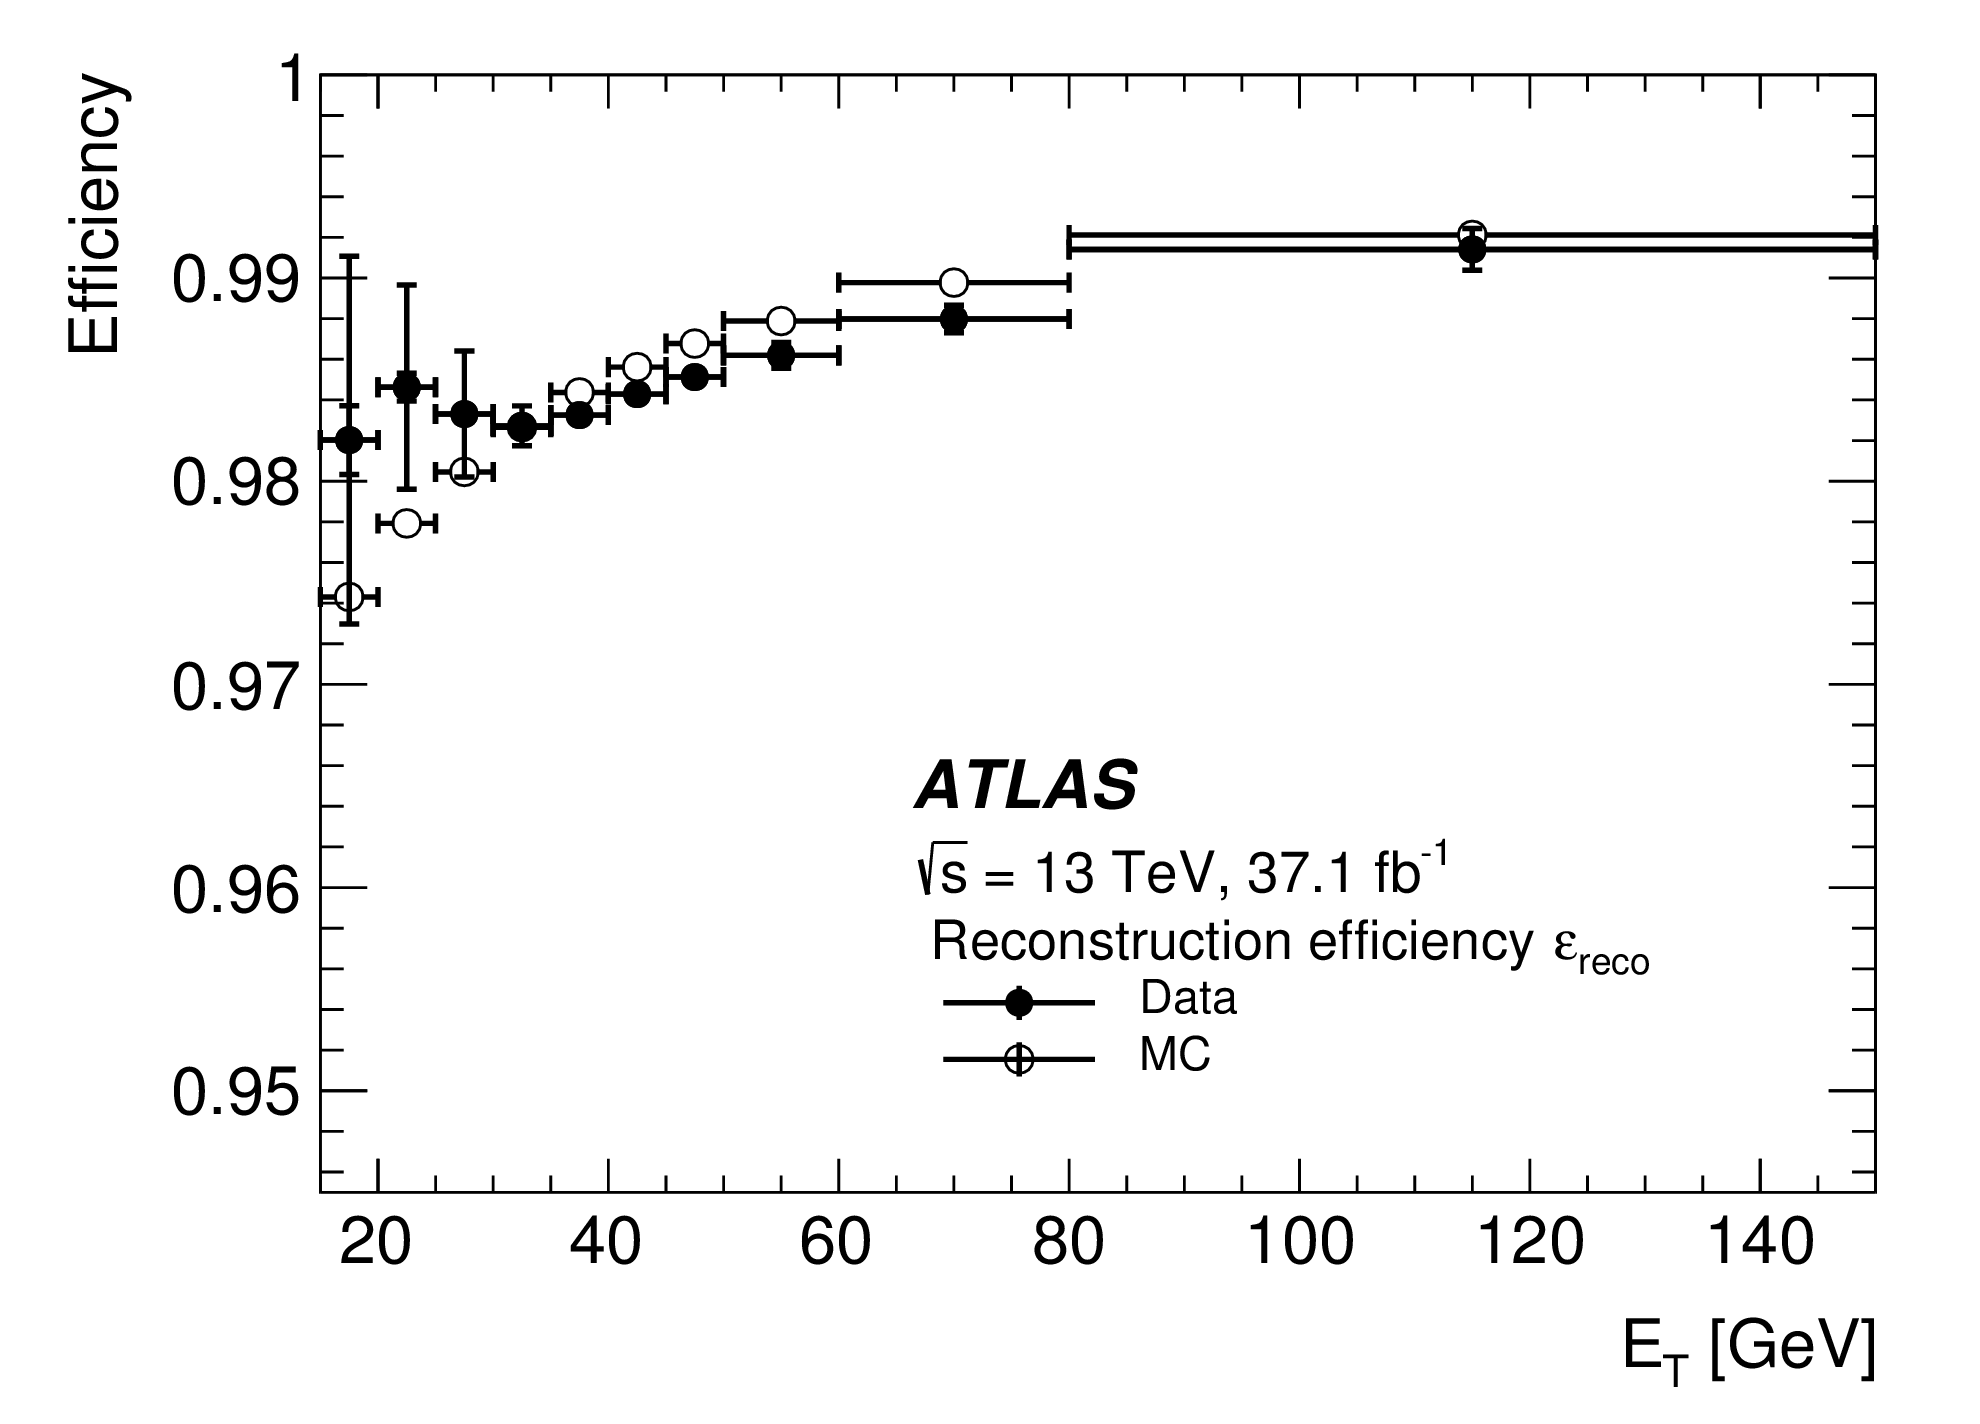
\includegraphics[width=0.48\textwidth]{figures/chapter3/egamma/egamma_reco_eff_Et}}
        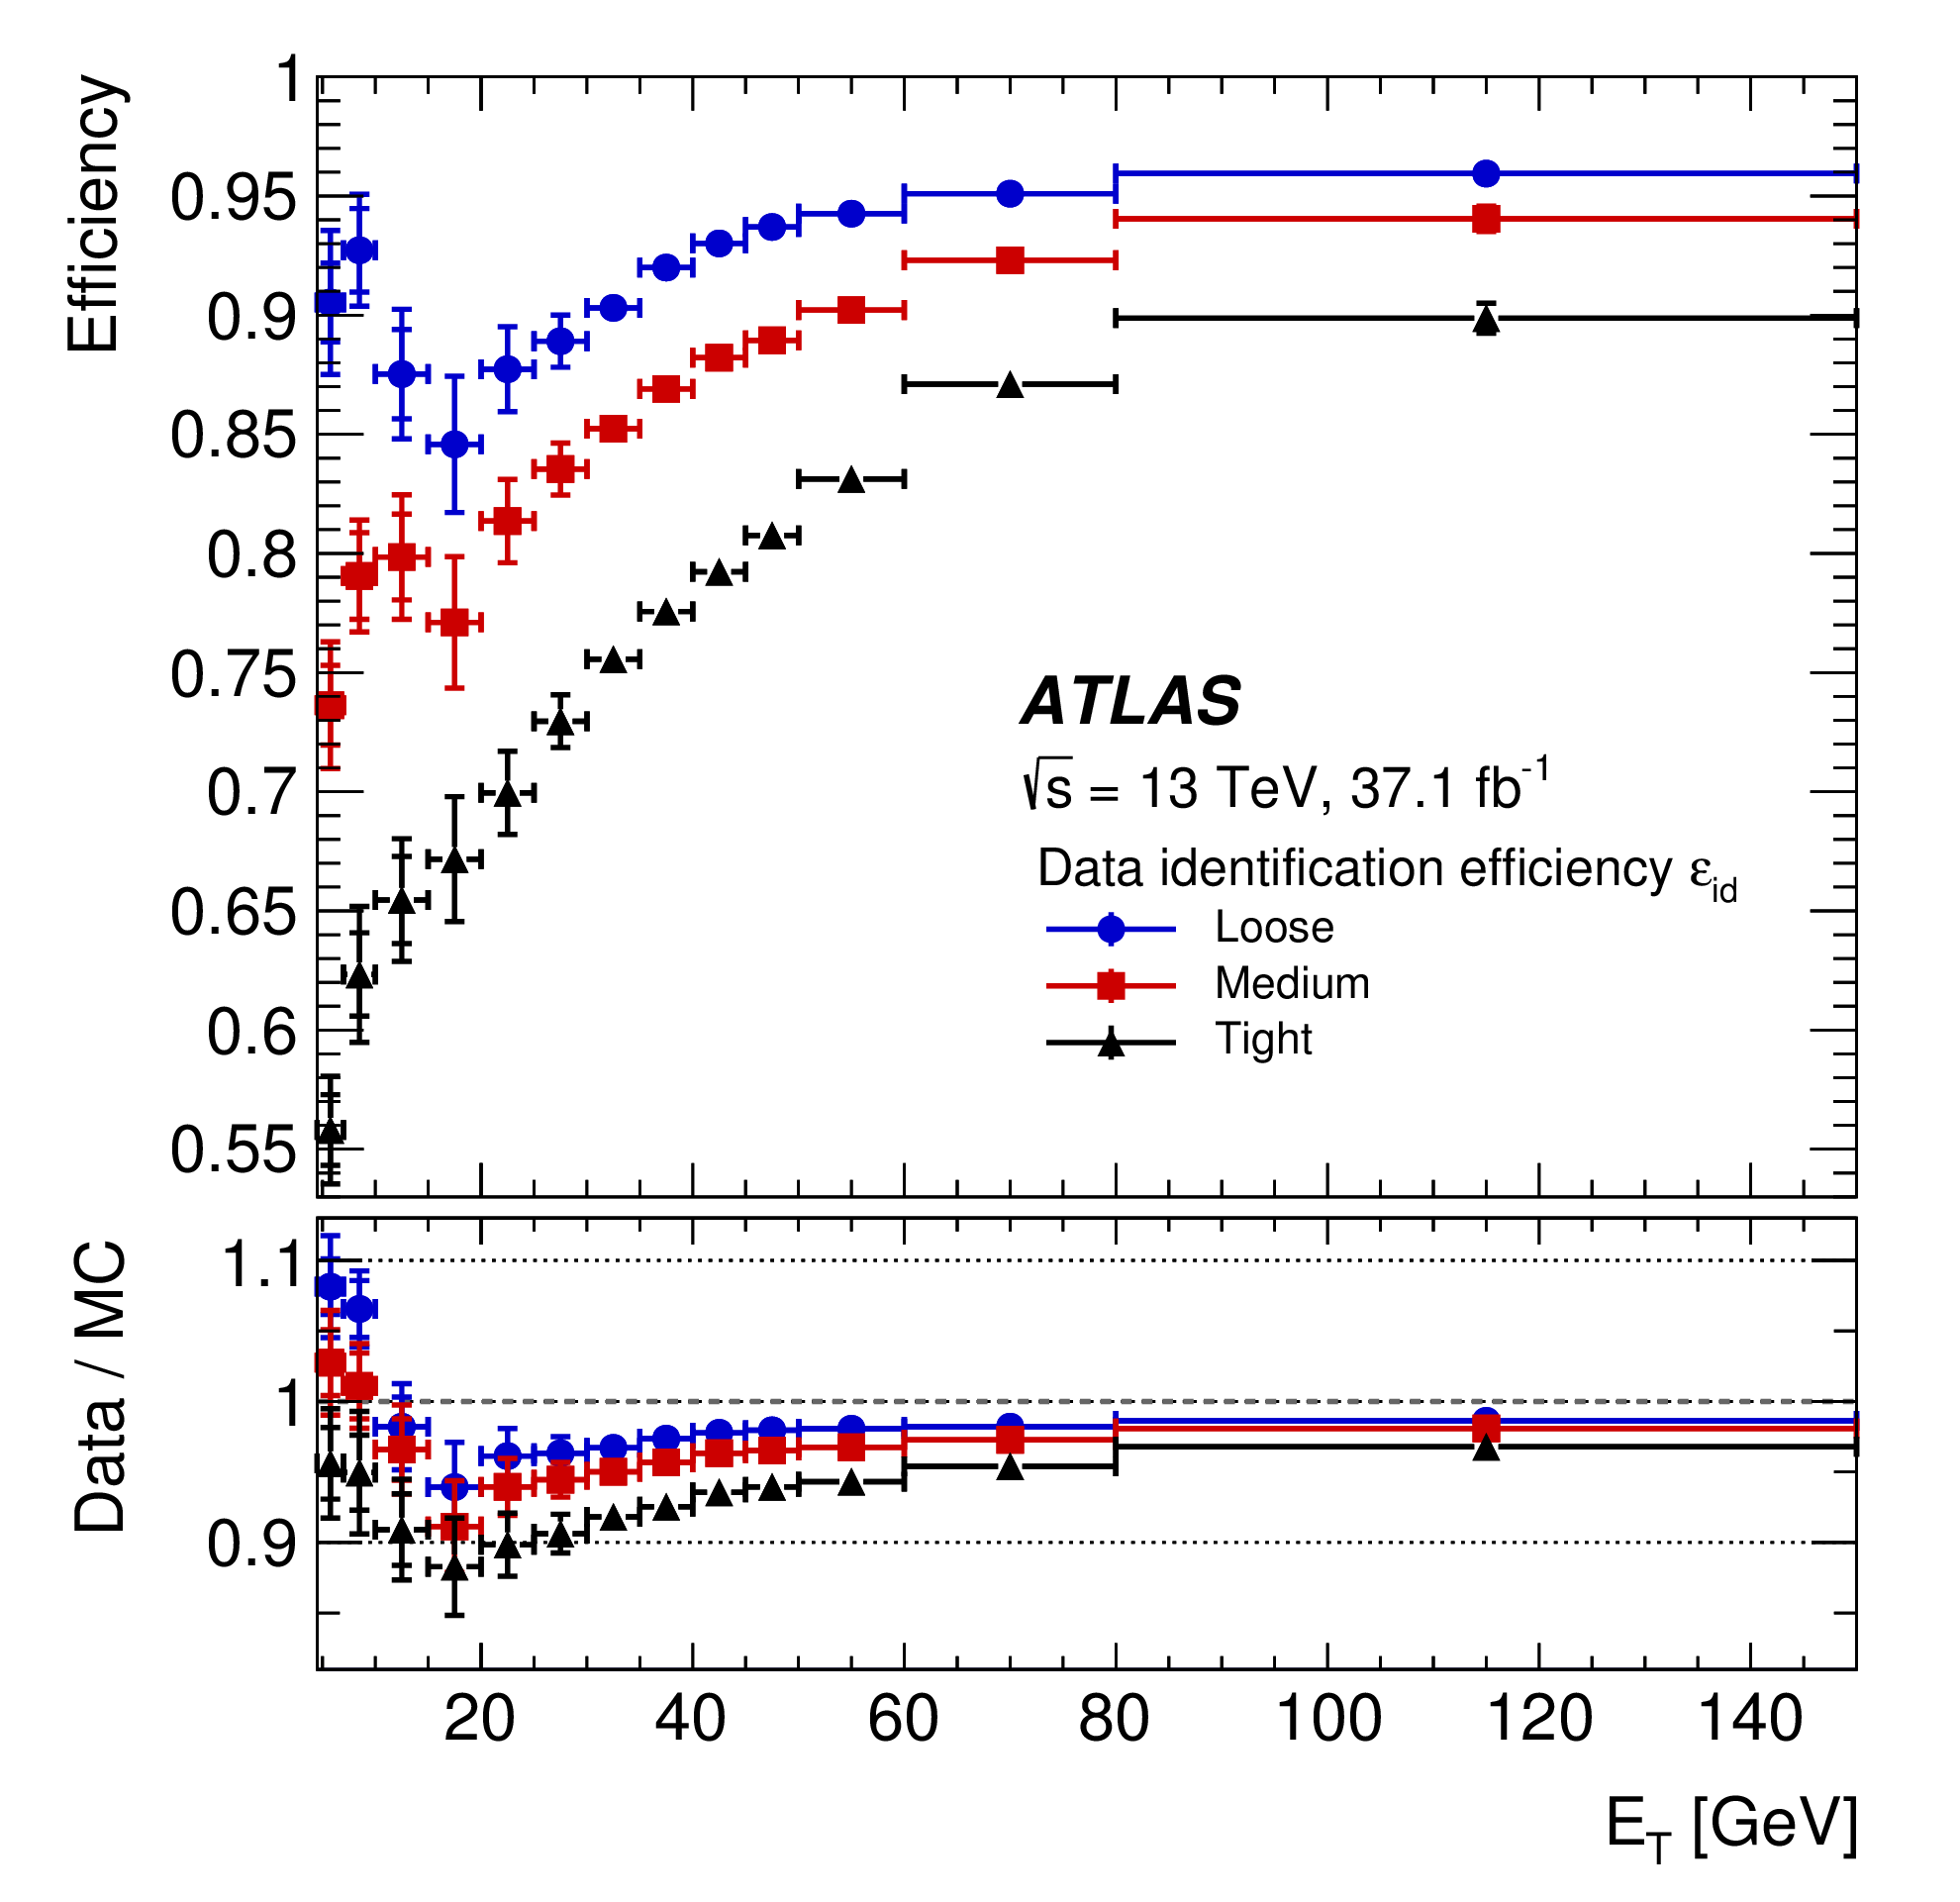
\includegraphics[width=0.48\textwidth]{figures/chapter3/egamma/egamma_id_eff_Et}
        \caption{
            {\color{red}{2015-2016}}
            \textbf{\textit{Left}}: Electron candidate reconstruction efficiency, measured in simulation and in data, as
                a function of the candidate $E_T$.
            \textbf{\textit{Right}}: Electron identification efficiency measured in data, as a function of electron $E_T$,
                for the three standard LH identification working points \textsc{Loose} (blue), \textsc{Medium} (red), and \textsc{Tight} (black).
                The lower panel shows the ratio of the efficiency measured in data over that measured in simulation.
        }
        \label{fig:egamma_eff_Et}
    \end{center}
\end{figure}

\subsection{Muons}
\label{sec:muons}

\subsubsection{Muon Reconstruction}
\label{sec:muon_reco}

The reconstruction of muon candidates is performed by combining the tracking
capabilities of the ID and the MS~\cite{Aad:2016jkr}.
Muon reconstruction first starts with the independent reconstruction of
charged-particle tracks within the ID and the MS.
The independently formed tracks are subsequently combined to form a complete
track representing the traversal of a muon through the full detector.
The muon track in the ID is reconstructed like any other charged-particle track (Section~\ref{sec:tracks_and_vertices}).

Muon reconstruction within the MS starts with a pattern finding phase, looking for
hit patterns each of the muon chambers to then form track segments.
The track segments between different MS layers are then fit together to form muon track candidates.
At least two matching track segments are required in order to build a muon
track candidate, except in the transition region between the barrel and end-cap where
single track-segment candidates can be used.
Once a muon track candidate is formed from the combined segments, a global $\chi^2$ fit is
performed to improve the association of hits to each muon candidate.
The $\chi^2$ is repeated several times, removing outlying hits as necessary, until a
threshold is met for all associated hits.

There are several algorithms used to combine the muon track candidates in the ID and MS, each
using different sets of information related to the ID, MS, and calorimeters.
At the time of the current work, there are four standard combination algorithms used
each based on the subdetectors used in their construction:

\begin{itemize}
    \item{\textbf{Combined Muon (CB)}} This type of muon is formed with a global refit using all muon track candidate hits
        in the ID and the MS. Hits may be added or removed from the MS track candidate during the refit.
        Muons are reconstructed following an outside-in pattern recognition algorithm, in which the
        muon is first reconstructed in the MS and extrapolated inwards to the ID hits.
        A complementary, albeit non-standard, inside-out algorithm also exists.
    \item{\textbf{Segment-tagged Muon (ST)}} An ID track is classified as a muon if, once extrapolated to the MS,
        it is associated with at least one local track segment in the MDT or CSC chambers. Segment-tagged muons
        are used when a muon candidate crosses only one layer of the MS chambers, either because of their
        low \pT~or because they fall into un-instrumented regions of the MS.
    \item{\textbf{Calorimeter-tagged Muon (CT)}} An ID track is classified as a muon if it is matched to an
        energy deposit in the caloriemter that is compatible with a minimum ionising particle.
        Calorimter-tagged muons have the lowest purity, but recover acceptance in regions of the MS
        that are only partially instrumented to allow for cabling and services to the calorimeter and ID systems,
        particularly in the region $\lvert \eta \rvert < 0.1$.
    \item{\textbf{Extrapolated Muon (ME)}} This type of muon is based only on the track candidates formed in the MS
        and a loose requirement that the track candidate be pointing back towards the IP.
        Extrapolated muons are mainly used to extend the acceptance of muon reconstruction into the region
        $2.5 < \lvert \eta \rvert < 2.7$ that is not covered by the ID acceptance.
\end{itemize}

\subsubsection{Muon Identification}
\label{sec:muon_id}

Muon identification refers to the act of applying aditional quality criteria on
the reconstructed muon candidates in order to mainly suppress contamination from
background sources that mimic muon signatures, such as pion and kaon decays, 
while ensuring high rates for the acceptance of prompt muons.
There are three standard muon identification working points in ATLAS, each
a subset of the previous one, and are referred to as the \textsc{Loose},
\textsc{Medium}, and \textsc{Tight} muon identification working points.
\textsc{Medium} muons are the default in ATLAS analyses and can only be composed
of CB and ME muons.
As all muons used in the present thesis are \textsc{Medium} muons, only this
identification working point will be described in detail.

Reconstructed muon candidates originating from non-prompt sources such
as in-flight decays of charged hadrons in the ID, are often characterised by the
presence of a `kink' in the reconstructed muon's track. It is therefore
expected that the independent momentum measurements made in the ID and MS may
be incompatible for non-prompt sources of muon candidates.
The muon identification criteria, then, make use of quantities
that relate the ID and MS muon track candidates.
These quantities are described in Table~\ref{tab:muon_id_vars}.
\textsc{Medium} muons have a rather loose selection on the compatibility between
the ID and MS momentum measurements and, with respect to those quantities in Table~\ref{tab:muon_id_vars},
are only required to have a $q/p$ significance less than 7.
On top of requirements on those quantities described in Table~\ref{tab:muon_id_vars},
the muon identification working points place
additional requirements on the number and type of hits in the ID and MS.
All identification working points require, in the ID, that there be at least 1 hit
in the pixel subdetector, at least 5 hits in the SCT subdetector, less
than 3 silicon holes,\footnote{A missing hit is considered a `hole' only
if it falls between hits successfully assigned to a given track.}
and at least 10\% of the TRT hits originally assigned to the muon track candidate exist
after the combined reconstruction.
\textsc{Medium} muons further require that the CB muons have at least 3 hits in at least
two MDT layers, except in $\lvert \eta \rvert < 0.1$ where tracks with at least one MDT layer but no more
than one MDT hole are allowed. The ME \text{Medium} muons are required to have at least
3 MDT or CSC layer hits, and are employed only in $2.5 < \lvert \eta \rvert < 2.7$.
{\color{red}{reference n MDT/CSC hits figure?}}


\begin{table}[!htb]
    \begin{center}
        \begin{tabularx}{\textwidth}{l|X|X}
        \hline
        \hline
        \textbf{Quantity Name} & \textbf{Measurement} & \textbf{Description} \\
        \hline
        $q/p$ significance & $\lvert (q/p)^{\text{ID}} - (q/p)^{\text{MS}} \rvert / \sqrt{ \sigma_{p_T}^{\text{MS}} + \sigma_{p_T}^{\text{ID}}}$ &
                Absolute value of the difference between the ratio of the charge and momentum of the muon candidates measured in the ID and MS,
                divided by the quadrature sum of the corresponding uncertainties. \\
        \hline
        $\rho^{\prime}$ & $\lvert p_T^{\text{MS}} - p_T^{\text{ID}} \rvert / p_T^{\text{Combined}}$ &
                Absolute value of the difference between the transverse momentum measurements in the ID and the MS,
                divided by that of the combined muon candidate. \\
        \hline
        $\chi^2_{\text{norm}}$ & -- & Normalized $\chi^2$ of the combined muon track fit \\
        \hline
        \hline
        \end{tabularx}
    \end{center}
    \caption{
    }
    \label{tab:muon_id_vars}
\end{table}

\begin{figure}[!htb]
    \begin{center}
        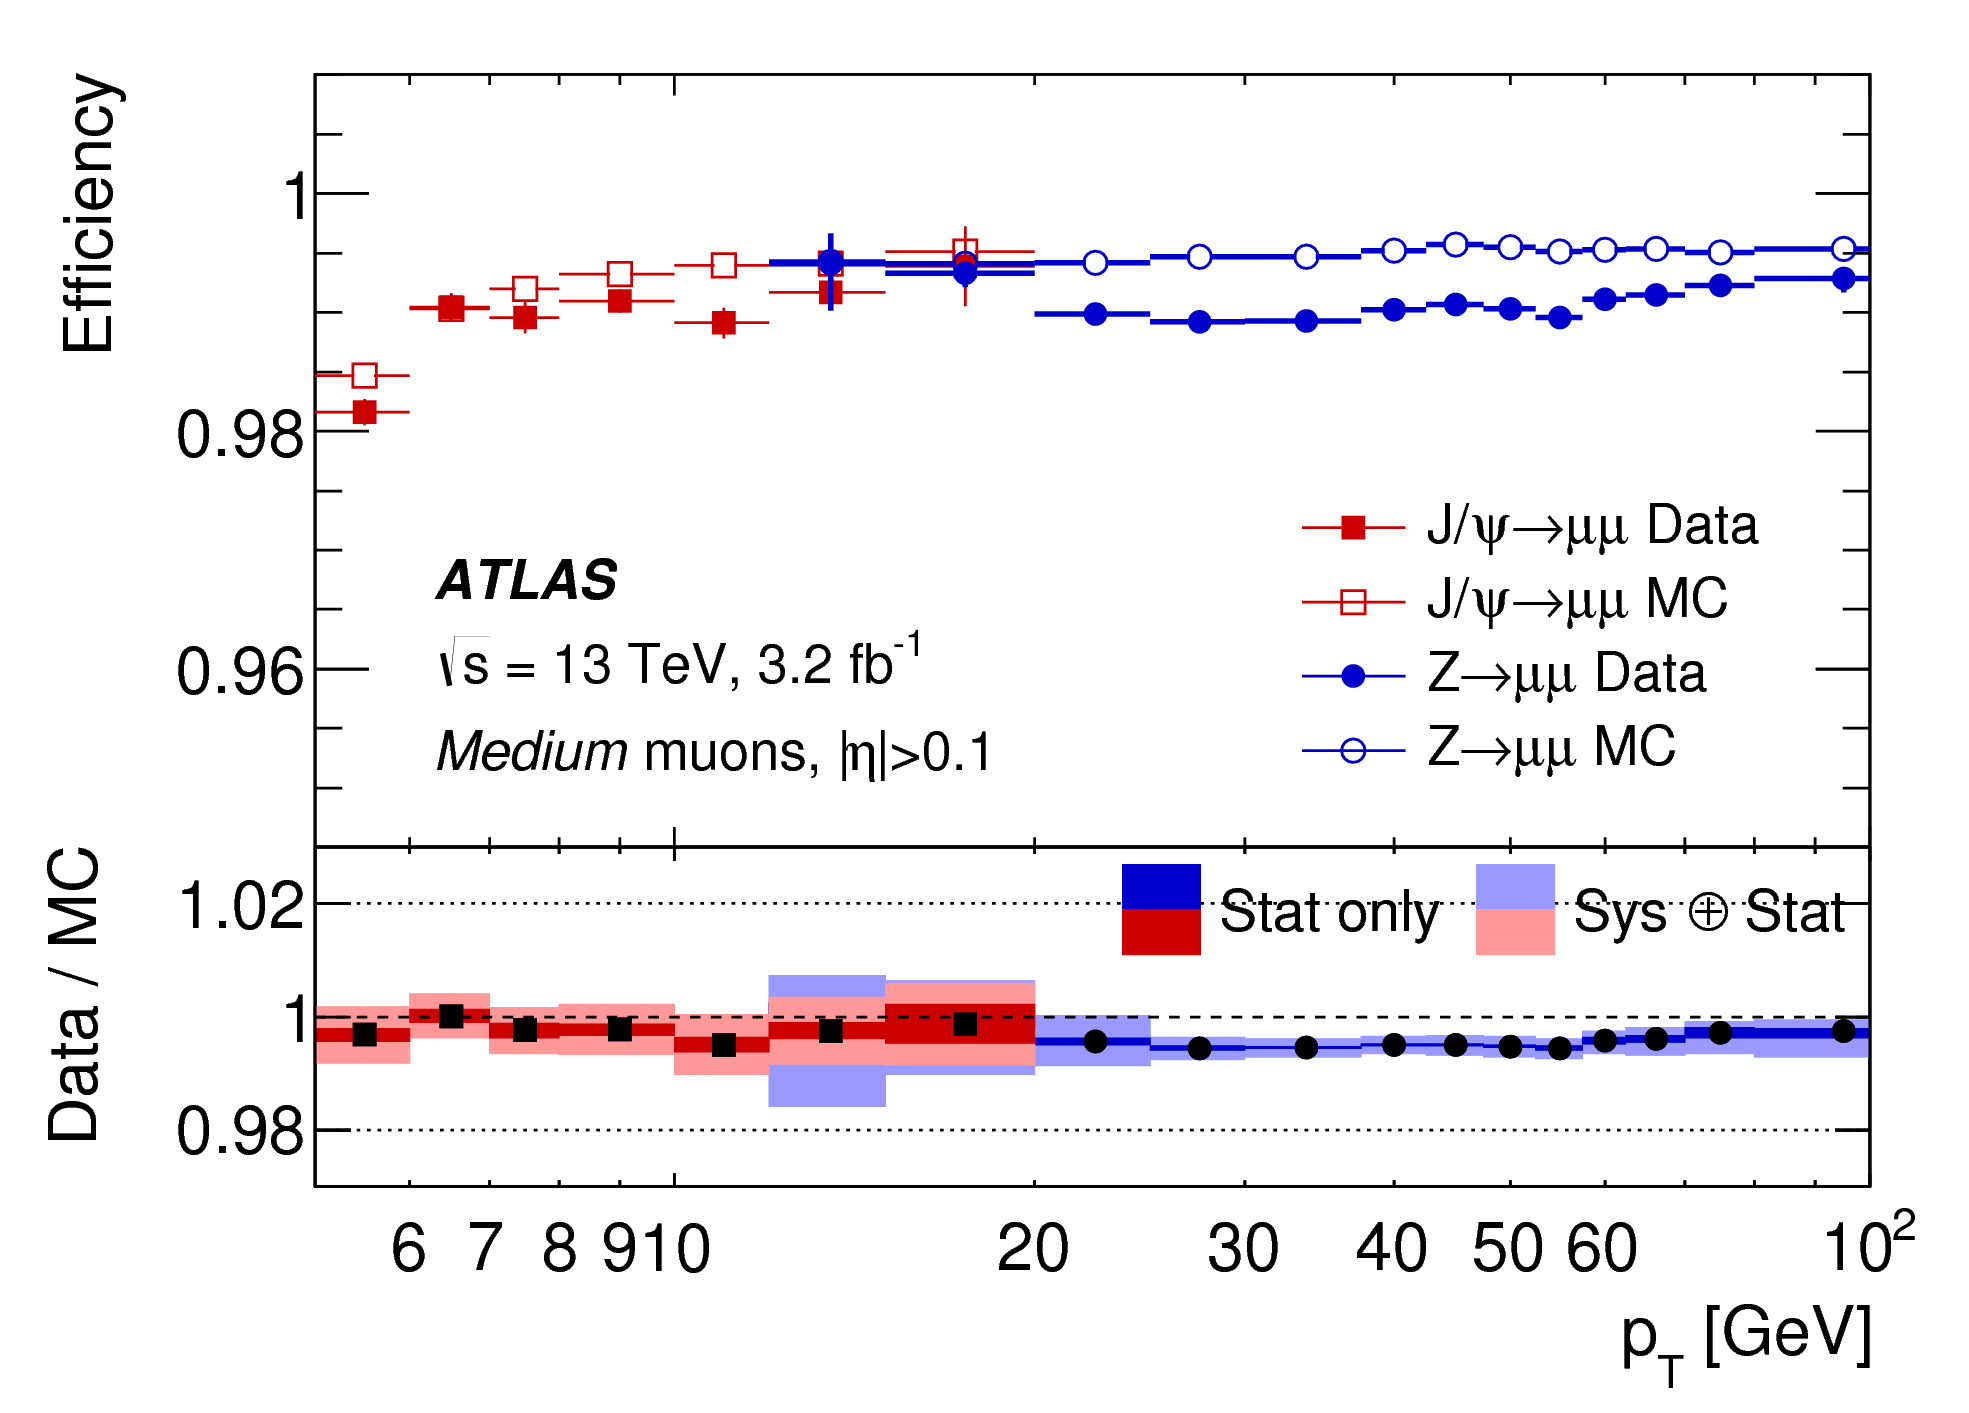
\includegraphics[width=0.7\textwidth]{figures/chapter3/muon/muon_reco_eff_medium}
        \caption{
            From Ref.~\cite{Aad:2016jkr}.
        }
        \label{fig:muon_reco_eff}
    \end{center}
\end{figure}

\FloatBarrier



%%%%%%%%%%%%%%%%%%%%%%%%%%%%%%%%%%%%%%%%%%%%%%%%%%%%%%%%%%%%%%%%%%%
%%%%%%%%%%%%%%%%%%%%%%%%%%%%%%%%%%%%%%%%%%%%%%%%%%%%%%%%%%%%%%%%%%%
% JETS
%%%%%%%%%%%%%%%%%%%%%%%%%%%%%%%%%%%%%%%%%%%%%%%%%%%%%%%%%%%%%%%%%%%
%%%%%%%%%%%%%%%%%%%%%%%%%%%%%%%%%%%%%%%%%%%%%%%%%%%%%%%%%%%%%%%%%%%
\section{Jets}
\label{sec:jets}

Due to the confining nature of QCD, color-charged quarks and gluons produced in the
initial $pp$ interactions do not exist as free states for observably meaningful
timescales and therefore do not leave unambiguous signatures in the detector.
Instead, their production is characterised by the radiation of additional
quarks and gluons roughly collinear with the initiating colored particles.
The radiation pattern of these colored objects is dictated by the color field
that binds them and eventually results in the production of color-neutral hadrons.
The collimated spray of hadrons as a result of this \textit{hadronisation} process
leads to the phenomenology of \textit{jets}, which are the macroscopically observable signature
of produced quarks and gluons.
The reconstruction of jets refers to any suitable, i.e. physically meaningful and stable,
method for grouping together, or \textit{clustering}, the end-products of the hadronisation
process in such a way that the properites of the initiating quarks or gluons, such
as their quantum numbers and/or kinematics, can be inferred from the resulting clustered object.
The standard method for reconstructing jets in ATLAS will be introduced in Section~\ref{sec:jet_reco}.
In Section~\ref{sec:jet_calib}, the steps taken to turn these reconstructed jets into
accurate representations of the initiating quarks and/or gluons, so that they can
be used meaningfully in physics analyses, will be discussed.

\begin{figure}[!htb]
    \begin{center}
        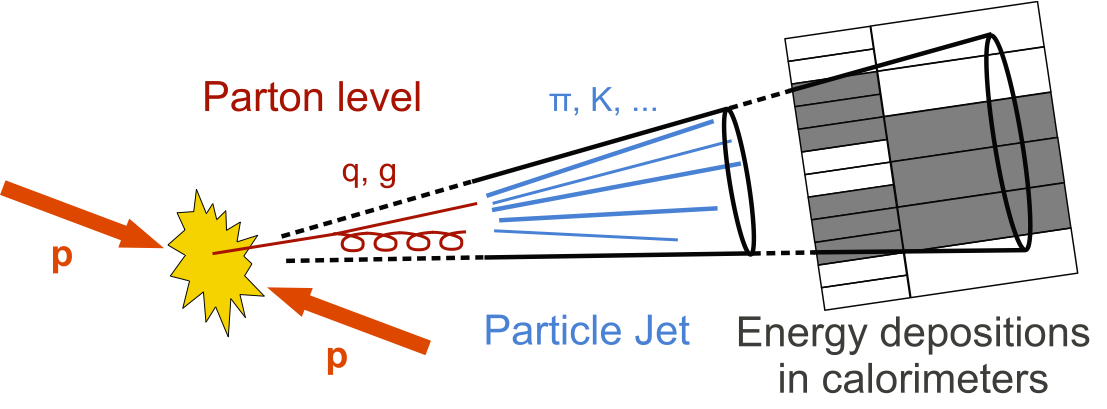
\includegraphics[width=0.7\textwidth]{figures/chapter3/jets/jet_formation_cartoon}
        \caption{
            Illustration of the jet formation process, beginning with the initiating quark and/or
            gluons (partons) which hadronise to form particle jets discernible by the tracking detectors
            in the ID and calorimeter jets defined by energy depositions in the calorimeter systems.
        }
        \label{fig:jet_formation}
    \end{center}
\end{figure}

\FloatBarrier
\subsection{Jet Reconstruction}
\label{sec:jet_reco}

\subsubsection{Topological Cell Clustering}
\label{sec:jet_topo_cluster}

The process of jet reconstruction begins first with the clustering of the lowest level calorimeter elements,
\textit{calorimeter cells}, corresponding to the readout channels in the LAr and tile calorimeters.
Figure~\ref{fig:calocell_granularity} gives an idea of the calorimeter cell granularity across the calorimeter
system.
The clustering algorithm used by ATLAS is a three-dimensional \textit{topological clustering} algorithm~\cite{Lampl:2008zz,Aad:2016upy}.
The highly granular calorimeter system used in ATLAS, with its finely segmented lateral readout and longitudinal sampling layers,
allows for the subsequent topological clusters (`topo-clusters') to capture in detail the energy-flow details of jets.
Topo-cluster formation begins by first identifying so-called \textit{seed cells} which have a rather high signal-to-noise ratio ($S/N$),
$S/N>4$.
Here, the signal is defined as the absolute value of the calorimter-cell energy measurement, $\lvert E \rvert$,
and the noise is defined as the sum in quadrature of the RMS of the electronics and expected pileup noise contributions.
Cells neighboring the seed cells satisfying $S/N>2$ are then collected into the topo-cluster.
A neighboring cell is defined in three-dimensions as either the calorimeter cells directly adjacent within the same calorimeter layer as
the seed cell, or, if in adjacent layers or in different calorimeter sub-systems, cells having at least partial overlap
in the $(\eta,\phi)$ plane with the seed.
The final set of cells, the perimeter cells, satisfying $S/N\ge0$ are then collected.
This last threshold essentially collects all those cells surrounding already-collected cells within each layer.
Figure~\ref{fig:calocell_clustering} illustrates the concept of topological cell clustering as described here.

\begin{figure}[!htb]
    \begin{center}
        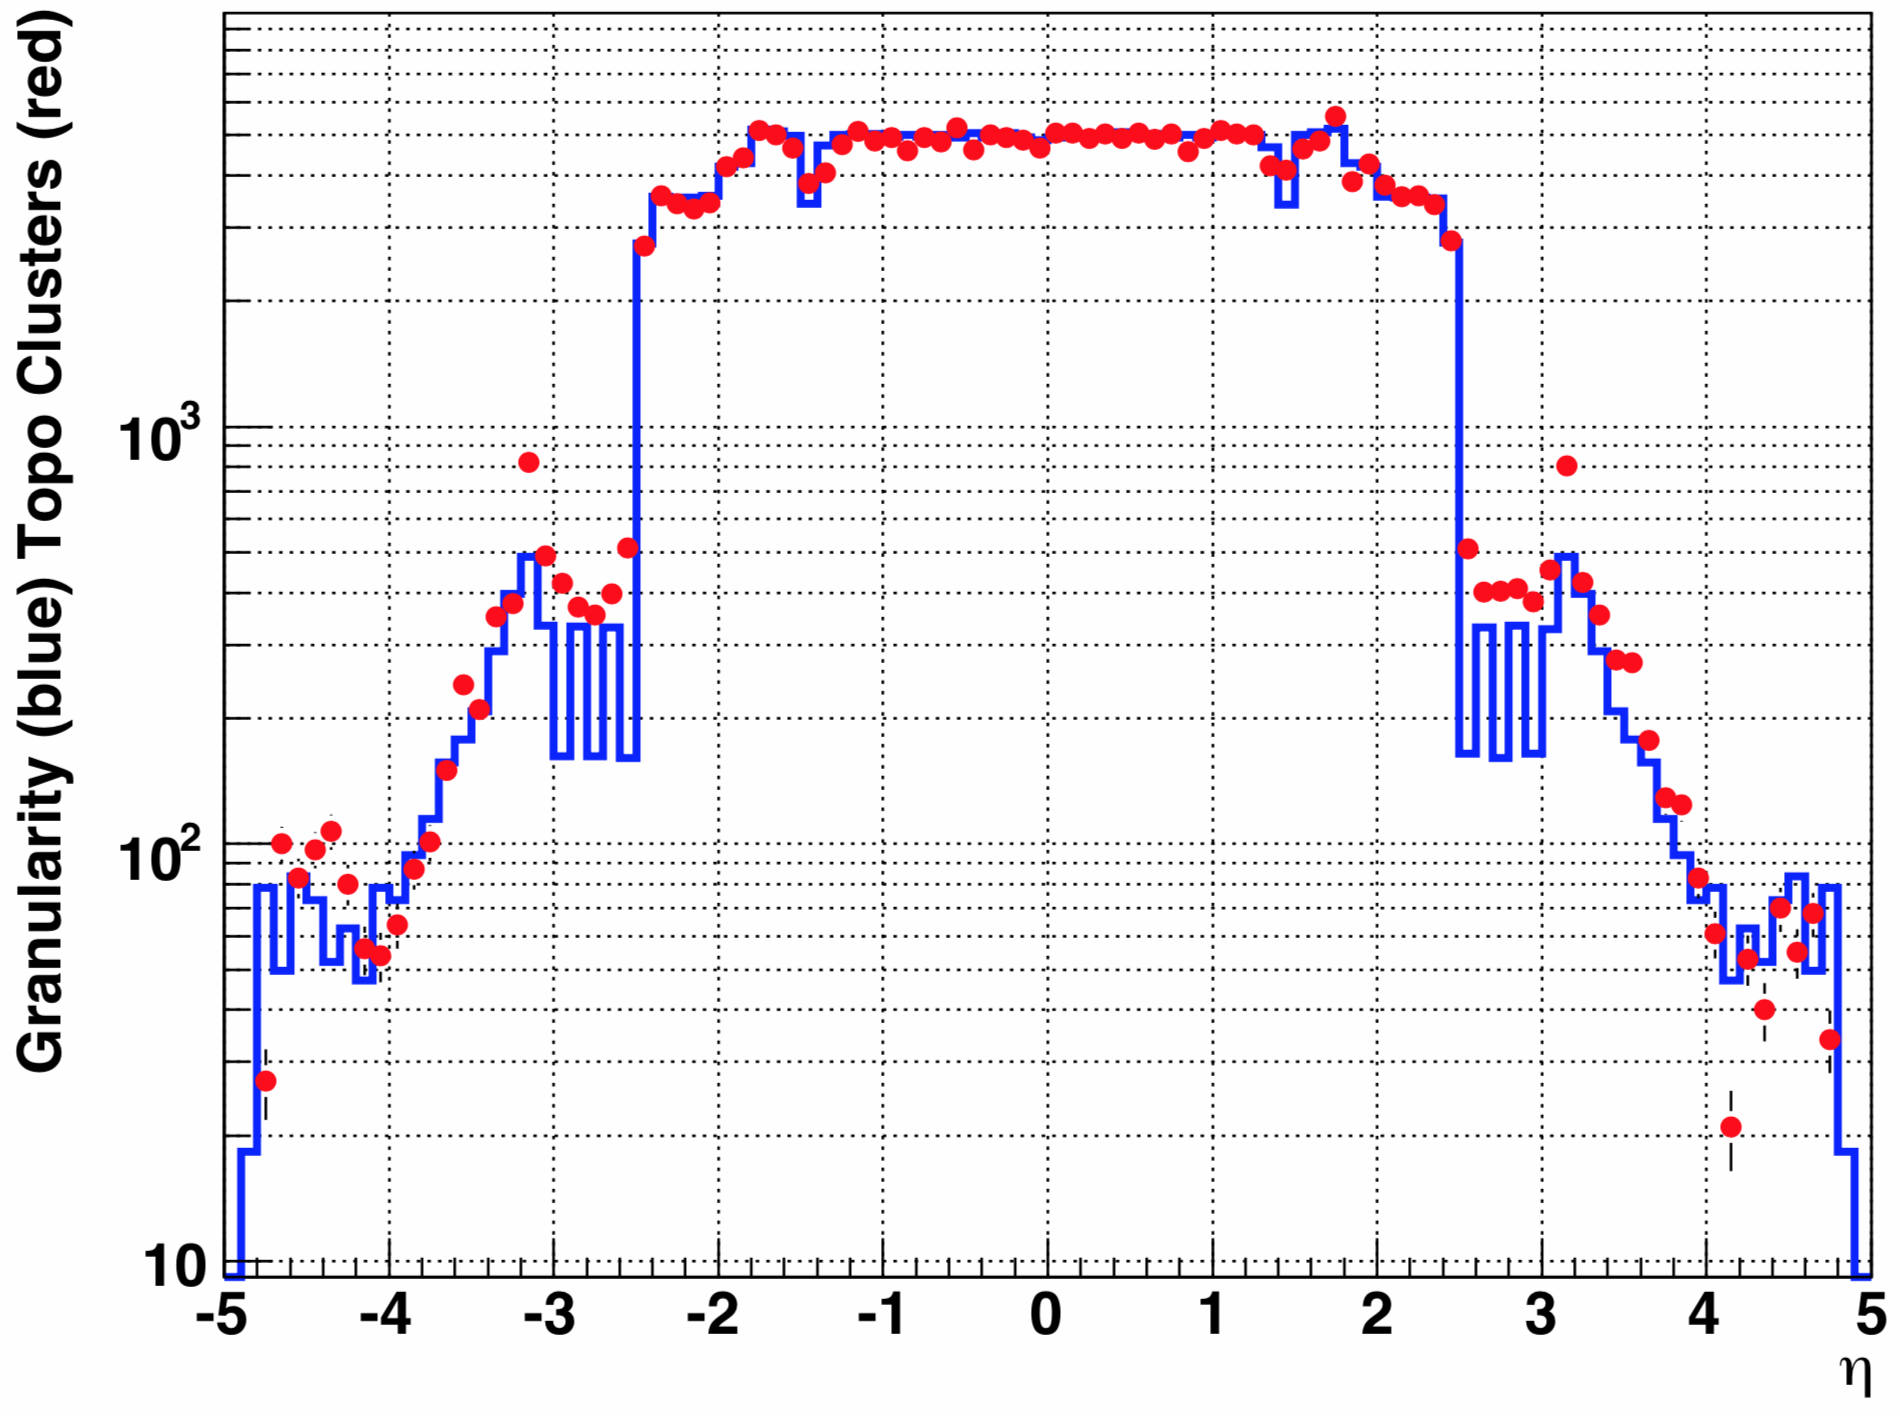
\includegraphics[width=0.5\textwidth]{figures/chapter3/jets/calocell_granularity}
        \caption{
            The blue histogram shows the average calorimeter cell granularity, i.e. number of calorimeter cells per
            $\Delta \eta = 0.1$, as a function of detector $\eta$. The red points show an approximation of the blue
            histogram based on calculations of the expected noise per calorimeter cell.
            From Ref.~\cite{Lampl:2008zz}.
        }
        \label{fig:calocell_granularity}
    \end{center}
\end{figure}

\begin{figure}[!htb]
    \begin{center}
    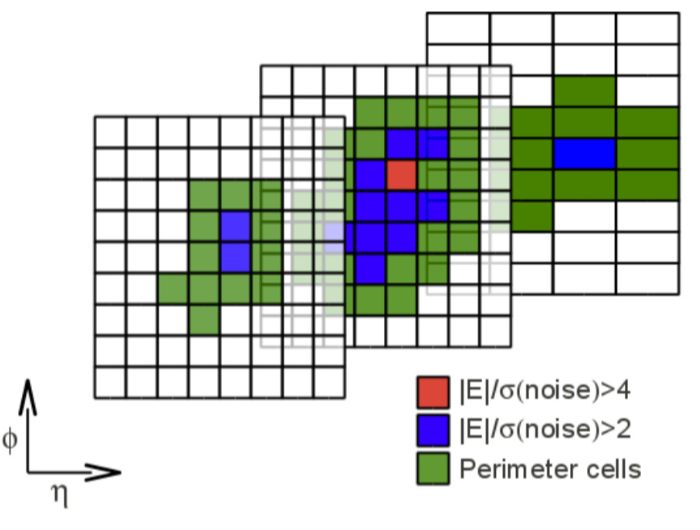
\includegraphics[width=0.6\textwidth]{figures/chapter3/jets/calocell_clustering_cartoon}
    \caption{
        Illustration of calorimeter-cell topological clustering across the three layers of the
        hadronic calorimeter. Indicated are the cells satisfying the signal-to-noise requirements for
        the seed (red), neighbor (blue), and perimeter (green) cells that make up the final three-dimensional topo-cluster.
    }
    \label{fig:calocell_clustering}
    \end{center}
\end{figure}
\FloatBarrier

\subsubsection{Jet Finding}
\label{sec:jet_finding}

Once the set of topo-clusters is formed, the process of jet finding begins.
As there is no single unique way to define a jet, there is a wide variety of jet finding algorithms whose
purpose is to associate jet constituents --- here, the calorimeter-cell topo-clusters --- to form
the final object representing the jet.
The default jet finding algorithm used by ATLAS is the
\textit{\antikt} jet clustering algorithm~\cite{Cacciari:2008gp}.
The \antikt~algorithm belongs to the more general class of sequential recombination algorithms
and is favored for its infrared and collinear (IRC) safe properties as well as the fact
that it tends to produce rather simple jets, geometrically, that are circular in the $\eta-\phi$ plane,
as seen in Figure~\ref{fig:antikt_circles}.
IRC safety in jet finding algorithms refers to the property that neither additional collinear splitting of jet constituents (e.g. the initiating or radiated partons)
nor soft emissions should change the clustered jet.
IRC-safe jets are therefore robust against these divergent regimes of QCD, sensitive to arbitrary
calculational choices made in perturbation theory, and makes them physically  meaningful observable objects
with which one can make predictions.

The \antikt algorithm takes as input constituents the topo-clusters described in Section~\ref{sec:jet_topo_cluster}
and computes the quantities,
\begin{align}
        d_{ij} = \min \left( \frac{1}{k^2_{T,i}} , \frac{1}{k^2_{T,j}} \right) \frac{ \Delta R_{ij}^2}{R^2},
        \label{eq:antikt_0}
\end{align}
\begin{align}
        d_{iB} = \frac{1}{k_{T,i}^2},
        \label{eq:antikt_1}
\end{align}
with $\Delta R_{ij}^2 = (\eta_i - \eta_j)^2 + (\phi_i - \phi_j)^2$, {\color{red}{its rapidity, right?}} $R$ is a parameter whose value regulates the radial extent of
the jet, and $k_{T,i}$ is the transverse momentum of the $i^{th}$ constituent.
The $d_{ij}$ and $d_{iB}$ quantities are `distance' metrics used in the clustering of input topo-cluster constituents.
The former represents the `distance' between the $i^{th}$ and $j^{th}$ constituent while latter represents the
`distance' between the $i^{th}$ consituent and the beam-line, introduced to distinguish between constituents
originating from the primary hard-scatter vertex and those originating from soft proton interaction remnants.
The work to be discussed in the present thesis sets $R=0.4$, which is the standard used in ATLAS.

The \antikt algorithm proceeds by clustering those constituents whose inter-distance is smallest, thereby tending to cluster
higher-\pT constituents together, which can be seen by inspection of Equation~\ref{eq:antikt_0} and \ref{eq:antikt_1}.
If, of the set of input constituents, the smallest distance is a $d_{ij}$, the associated constituents indicated by $i$
and $j$ are recombined to form a single constituent in the list that replaces them both.
If the smallest distance is a $d_{iB}$, then the constituent indicated by index $i$ is removed from the set of constituents
and is considered as a complete jet.
This process repeats, starting with the now smaller (due to successful constituent recombination or removal) set of constituents,
until no constituents are left.
The result of this process is a set of recombined constituents that represent jets, as illustrated in Figure~\ref{fig:antikt_circles}.

\begin{figure}[!htb]
    \begin{center}
        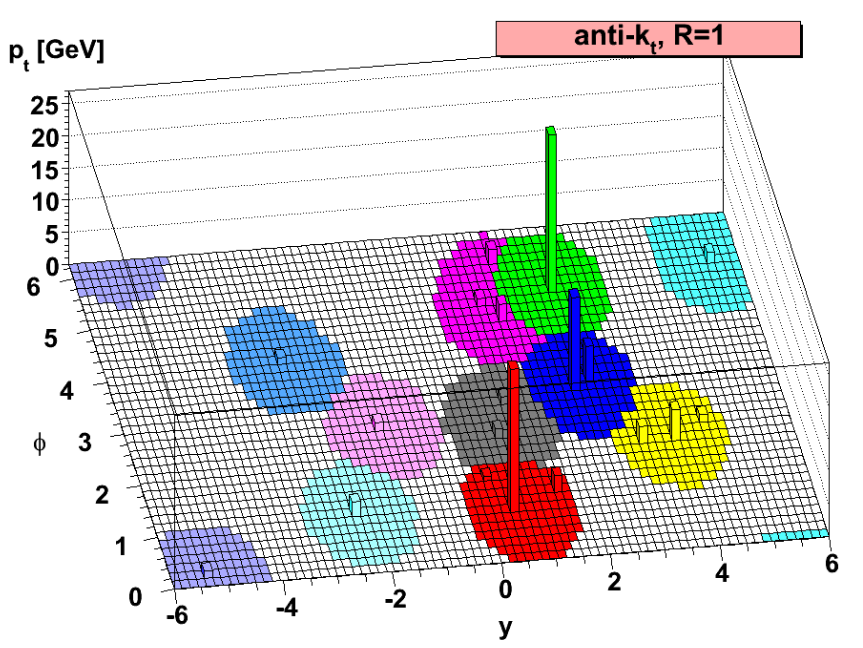
\includegraphics[width=0.5\textwidth]{figures/chapter3/jets/antikt_jet_circles}
        \caption{
            An illustration of jet constituents clustered by the \antikt~algorithm. Seen
            are the energetic constituents.
            The filled and colored circles represent areas populated by soft jet consituents, and represent the jet \textit{catchment area}~\cite{Cacciari:2008gn}
            whose size is dictated by the $R$ parameter in the \antikt algorithm (Equation~\ref{eq:antikt_0}).
            Figure taken from Ref.~\cite{Cacciari:2008gp}.
        }
        \label{fig:antikt_circles}
    \end{center}
\end{figure}

\FloatBarrier
%%%%%%%%%%%%%%%%%%%%%%%%%%%%%%%%%%%%%%%%%%%%%%%%%%%%%%%%%%%%%%%%%%%%%%%%%%%%%%%%%%%%%%%%%%%%%%%%%%
%%%%%%%%%%%%%%%%%%%%%%%%%%%%%%%%%%%%%%%%%%%%%%%%%%%%%%%%%%%%%%%%%%%%%%%%%%%%%%%%%%%%%%%%%%%%%%%%%%
%
% CALIBRATION
%
%%%%%%%%%%%%%%%%%%%%%%%%%%%%%%%%%%%%%%%%%%%%%%%%%%%%%%%%%%%%%%%%%%%%%%%%%%%%%%%%%%%%%%%%%%%%%%%%%%
%%%%%%%%%%%%%%%%%%%%%%%%%%%%%%%%%%%%%%%%%%%%%%%%%%%%%%%%%%%%%%%%%%%%%%%%%%%%%%%%%%%%%%%%%%%%%%%%%%


\subsection{Jet Calibration}
\label{sec:jet_calib}

\begin{figure}[!htb]
    \begin{center}
        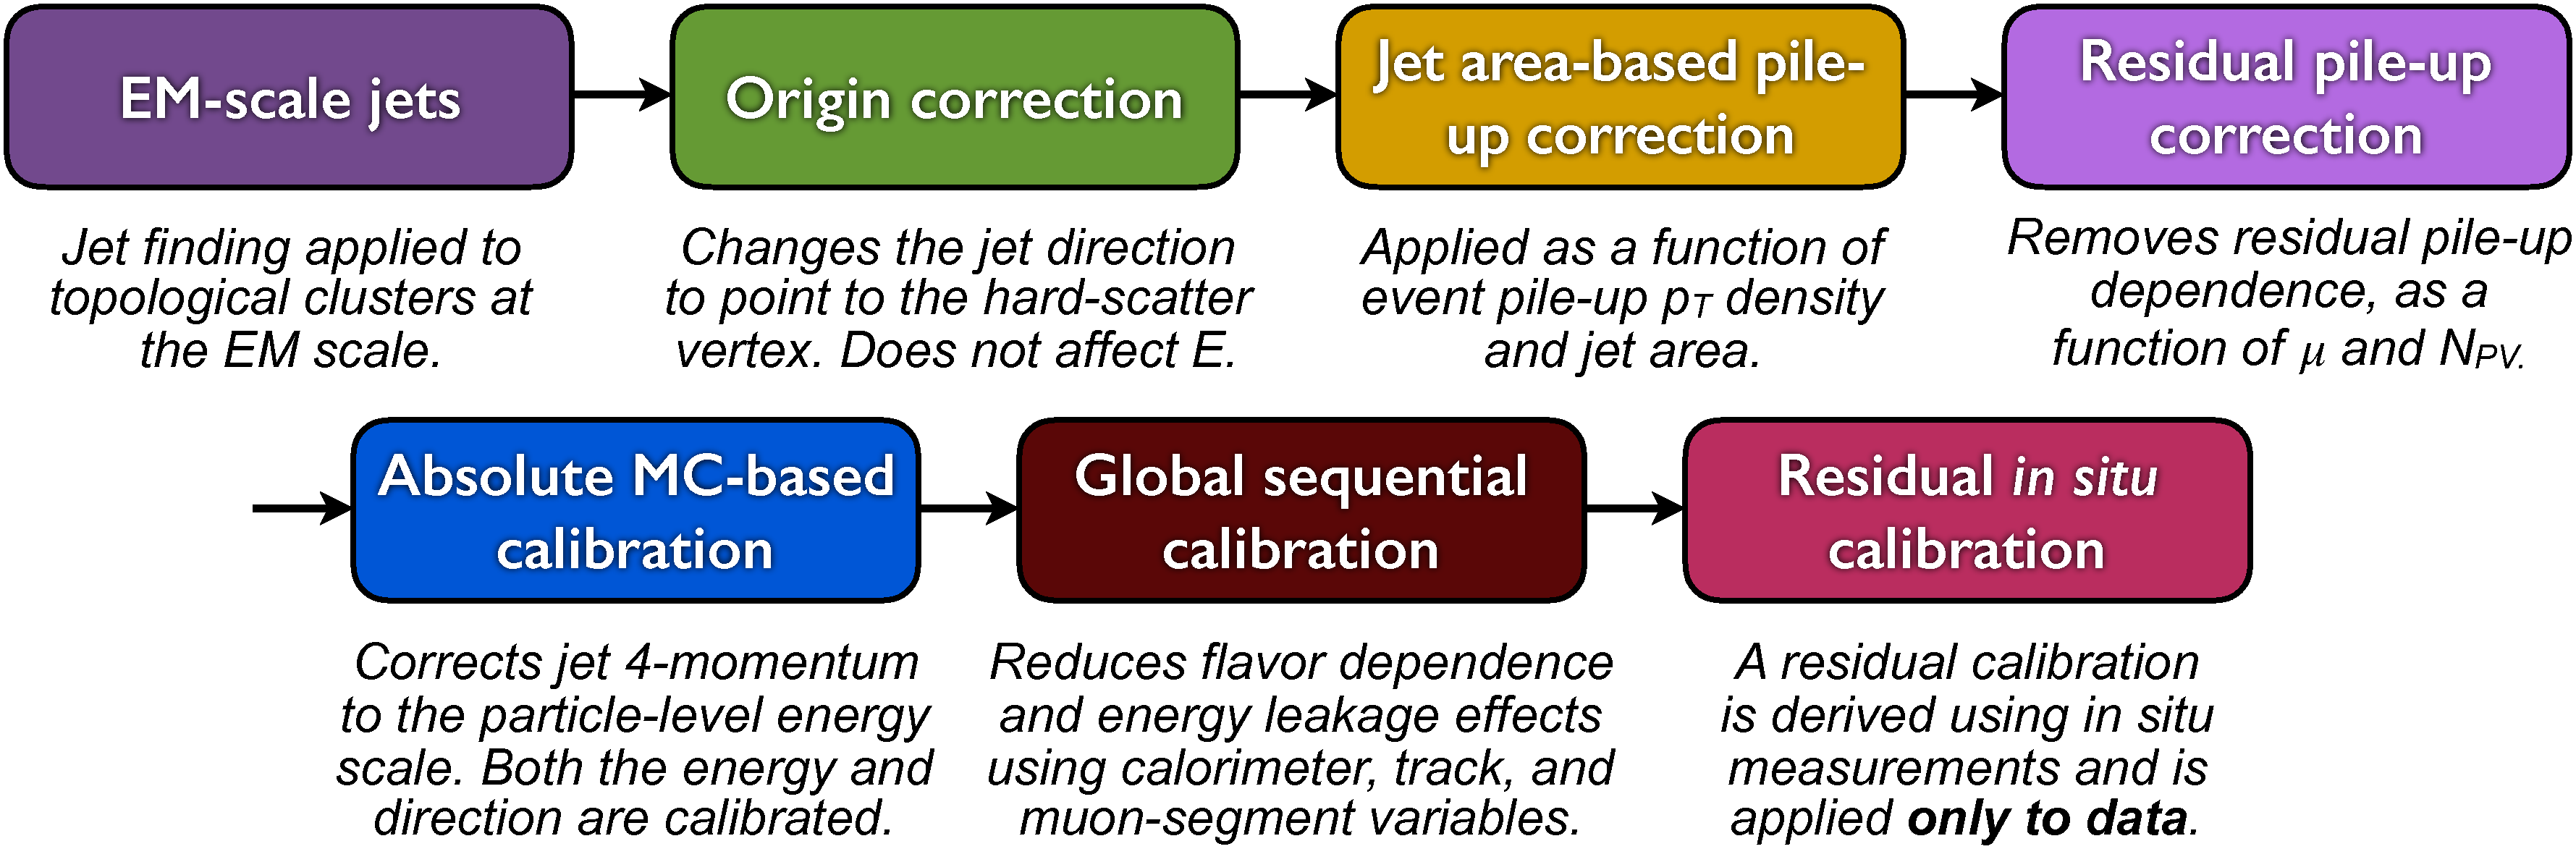
\includegraphics[width=0.8\textwidth]{figures/chapter3/jets/jes_calibration_sequence}
        \caption{
            From Ref.~\cite{Aaboud:2017jcu}.
        }
        \label{fig:jes_sequence}
    \end{center}
\end{figure}

The jets reconstructed following the steps described in Section~\ref{sec:jet_reco} are objects clustered
at the electromagnetic (EM) scale, which correctly measures the energy of electromagnetic showers but does not
accurately account for energy depositions arising as a result of hadronic shower growths.
These jets are therefore referred to as `EM-scale' jets.
To correctly assign meaningful energy and momentum measurements to the reconstructed jets that correspond
to the energies and momenta of the initiating, underlying particle-level jets, several \textit{jet energy scale} (JES) calibration steps are taken~\cite{Aaboud:2017jcu}.
The steps are detailed in the flowchart in Figure~\ref{fig:jes_sequence} and will be briefly described in the following text.
{\color{red}{After these steps.. jets are referred to as EM+JES scale jets...}}

\subsubsection{Jet Origin Correction}
\label{sec:jet_origin_correction}

The reconstructed EM-scale jets are built with the assumption that they originate from the geometric center
of the detector, as opposed to the primary hard-scatter vertex from which the initiating partons arise.
The so-called jet origin corretion, therefore, refers to recalculating the jet four-momentum vector by adjusting it
in such a way that it points to the primary hard-scatter vertex.
This correction acts primarily to improve the $\eta$ resolution of jets.
This procedure is only one hundred percent accurate, of course, under the assumption that all of the jet constituents
going into the EM-scale jet reconstruction originated from the hard-scatter vertex, as opposed to some fraction having come from
a pileup vertex, for example.

\subsubsection{Pileup Corrections}
\label{sec:jet_pileup_correction}

Jets are extended object with relatively large \textit{catchment areas}~\cite{Cacciari:2008gn} that make them susceptible to
pileup effects.
Several corrections, therefore, to the jet energy are taken in order to account for contributions to the EM-scale jet reconstruction
arising from both in-time and out-of-time pileup interactions.

The first pileup correction is an area-based correction which subtracts the per-event pileup contribution to the
\pT~of each jet based on the jet's area, where the jet area is defined as in Ref.~\cite{Cacciari:2008gn}.
This pileup contribution is taken as the median \pT~density, $\rho$, of jets in the $\eta-\phi$ plane and
can be thought of as a baseline `noise' term distributed evenly throught the calorimeter that contributes to a jet's reconstructed energy.
%The quantity $\rho$ depends on the pileup activity in the event and is taken as a function of the number of reconstructed
%primary vertices (\npv) in a given event; for example, the pileup density is expected to be larger for an event
%with $\npv = 25$ as compared to one with $\npv = 5$.

After the area-based pileup correction is made, there still remains residual dependence of the reconstructed jet \pT~on the
number of reconstructed primary vertices and on the number of interactions, $\mu$.
These dependences are measured by performing linear fits of the jet \pT~as a function of each quantity, binned as a function of the detector $\eta$, $\eta_{\text{det}}$.

The final, pileup-corrected jet \pT~is given by Equation~\ref{eq:jet_pileup_corr}:
\begin{align}
    \pT^{\text{Corr}} = \pT^{\text{Reco}} - \underbrace{\rho \times A}_{\text{Area-based}} - \underbrace{\alpha \times (\npv - 1) - \beta \times \mu}_{\text{Residual}},
    \label{eq:jet_pileup_corr}
\end{align}
where $A$ is the jet area, and the $\alpha$ and $\beta$ terms are derived from the linear fits mentioned above and are $\alpha = \partial \pT / \partial \npv$
and $\beta = \partial \pT / \partial \mu$, respectively.
The former accounts for effects arising as a result of in-time pileup and the latter for those due to out-of-time pileup.
The effect of the pileup corrections is shown in Figure~\ref{fig:jet_pileup_corr}, where it can be seen that the area-based correction
is an overall offset, as expected, after which residual pileup dependencies of the jet \pT~as a function of $\lvert \eta_{\text{det}} \rvert$ are still observed.
This residual pileup dependence is greater in the forward regions of the detector where pileup and background activity is largest.

\begin{figure}[!htb]
    \begin{center}
        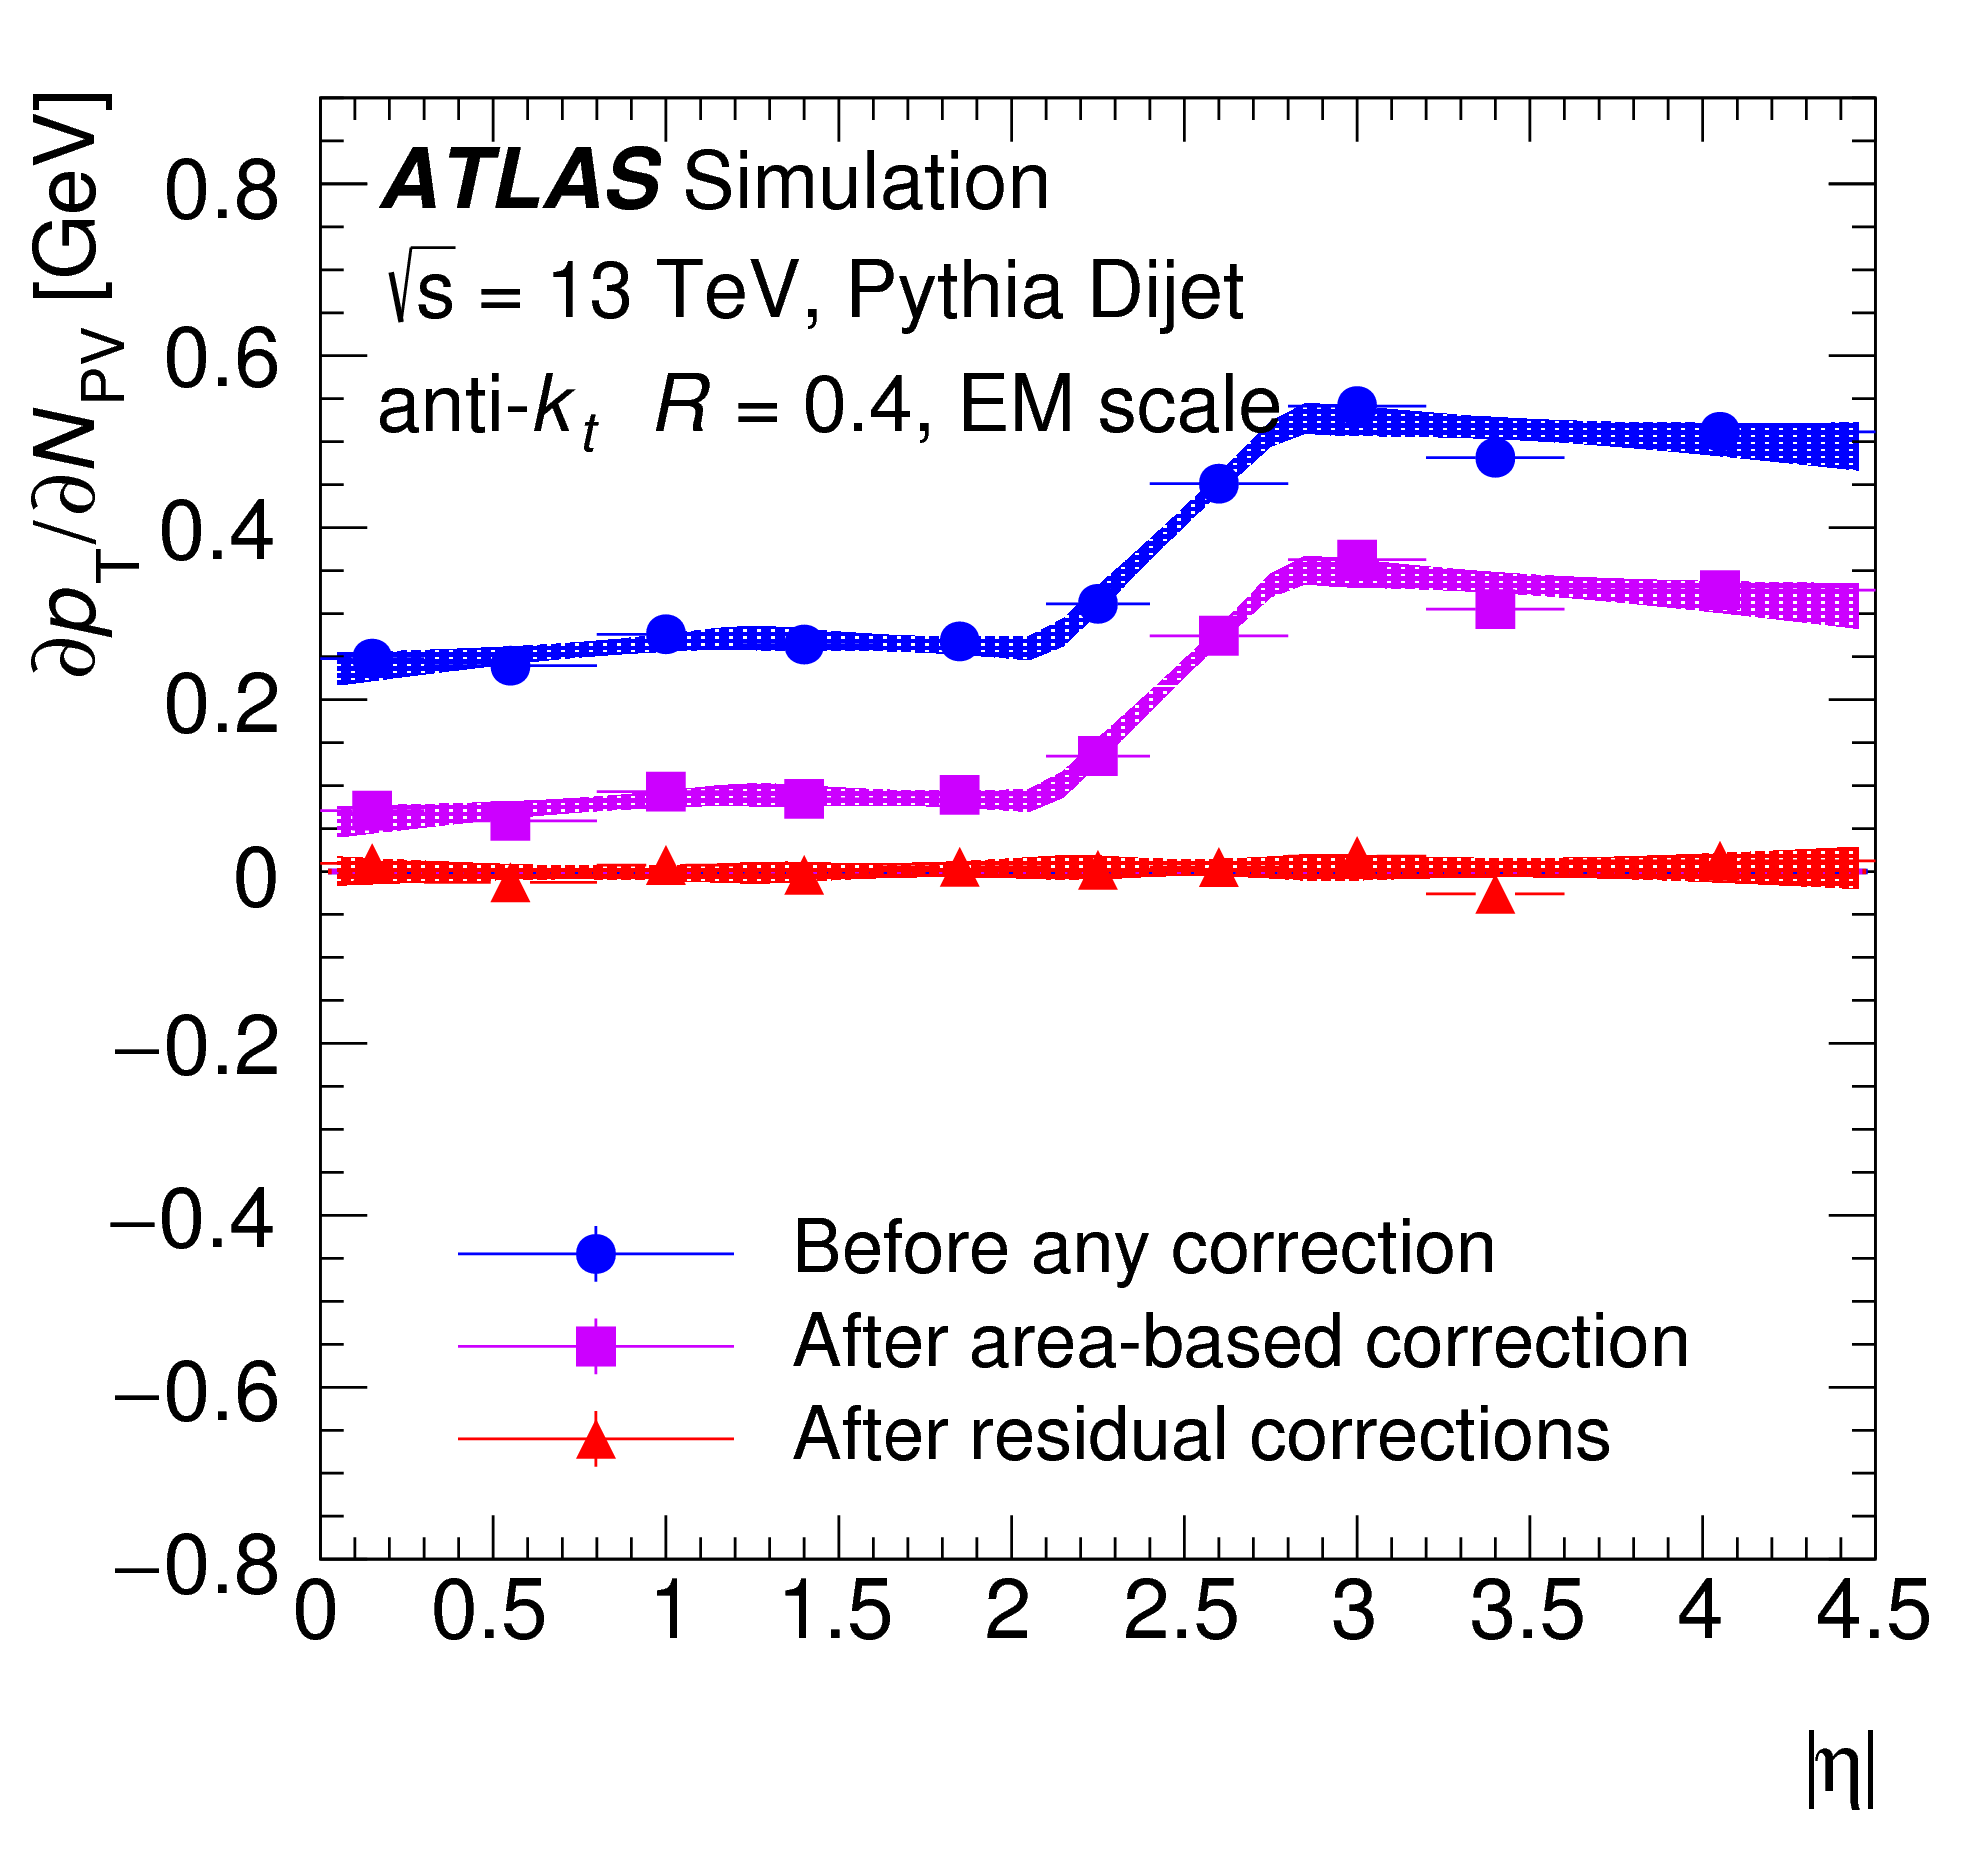
\includegraphics[width=0.4\textwidth]{figures/chapter3/jets/jet_pileup_corr_alpha}
        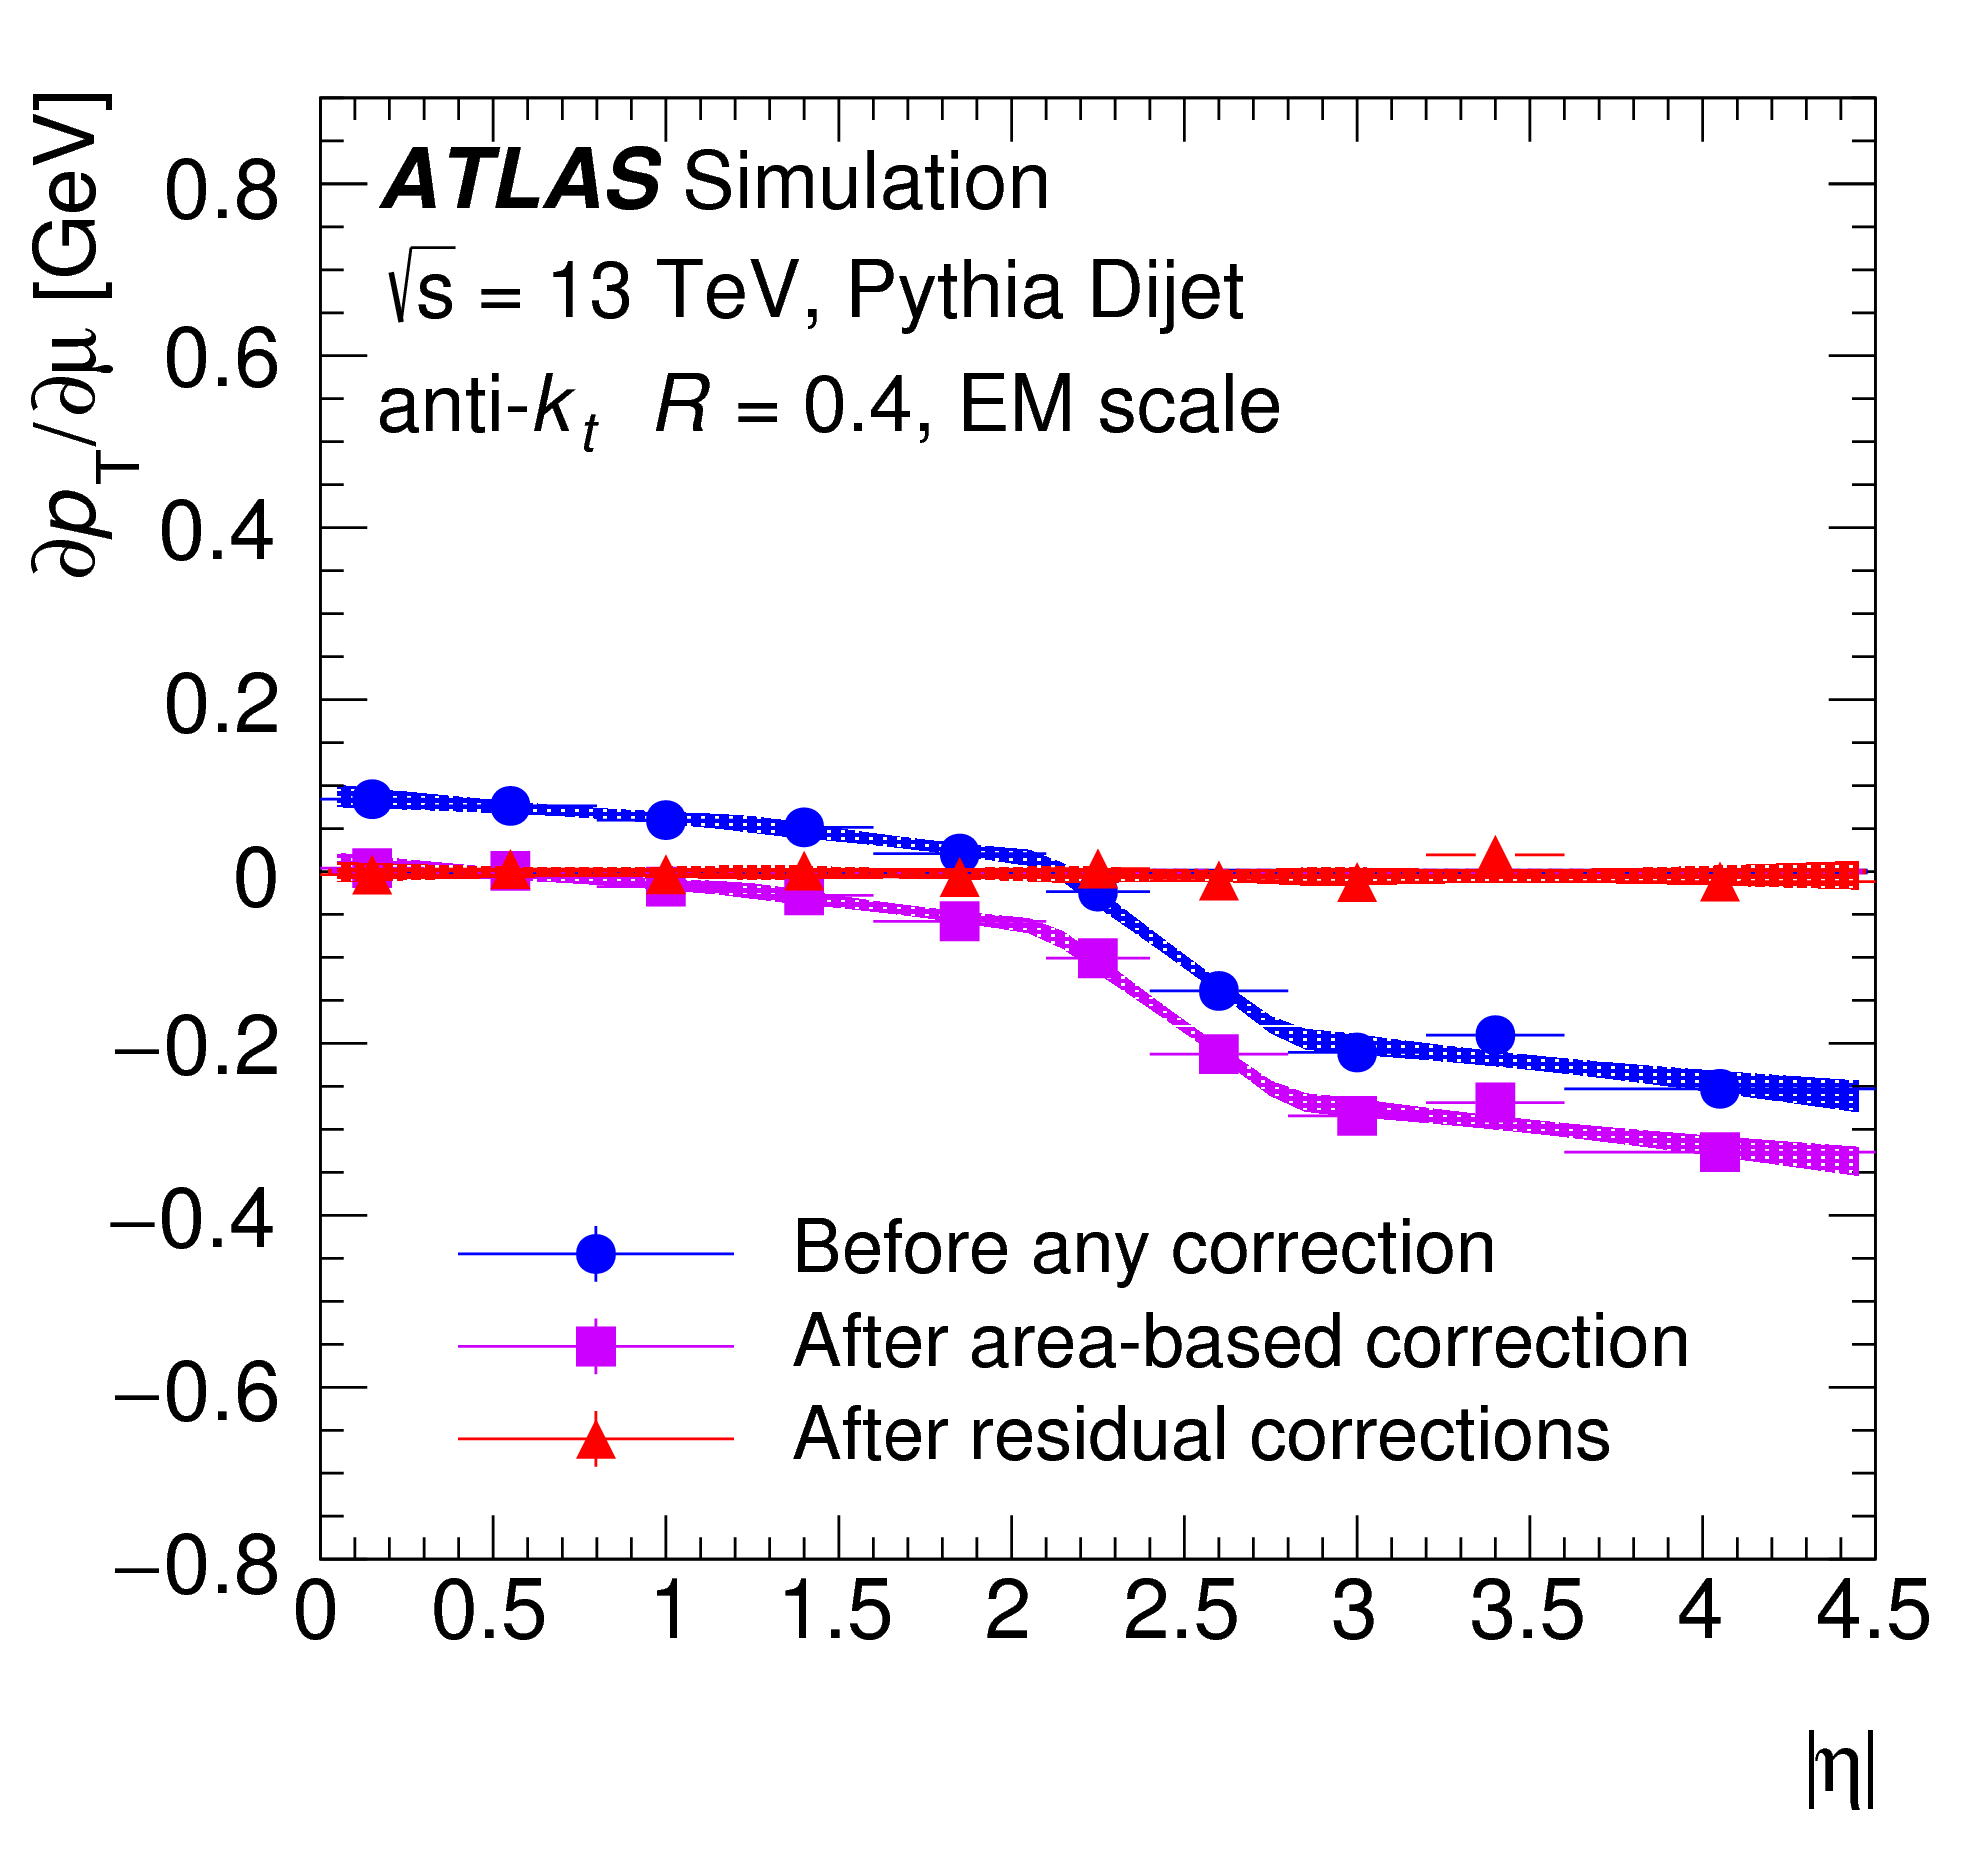
\includegraphics[width=0.4\textwidth]{figures/chapter3/jets/jet_pileup_corr_beta}
        \caption{
            Dependence of the \pT~of EM-scale reconstructed jets on \npv (in-time pileup) (\textit{left}) and on
            $\mu$ (out-of-time pileup) (\textit{right}).
            The blue curves show the dependence prior to any pileup corrections,
            the purple curves are after the area-based correction,
            and the red curves are the final dependence after the full pileup correction described in Equation~\ref{eq:jet_pileup_corr}
            is taken into account.
            Figures taken from Ref.~\cite{Aaboud:2017jcu}.
        }
        \label{fig:jet_pileup_corr}
    \end{center}
\end{figure}

\subsubsection{Absolute Jet Energy Scale and $\eta$ Correction}
\label{sec:jet_eta_corr}

This correction corrects the EM-scale reconstructed jet to the true energy scale based on particle-level
jets and is therefore purely MC-based.
Particle-level jets are jets clustered using the \antikt~algorithm but using the generator-level
particles at the end of the hadronisation step as the input constituents, and therefore represent the reconstructed jet prior to
its interaction with the calorimeter (see Figure~\ref{fig:jet_formation}).
The correction accounts for mismodelling of the inactive material within the detector, radiation not accounted for
in the reconstructed calorimeter-based jet due to the clustering algorithm not accepting it (`out-of-cone radiation`),
non-compensation of the hadronic calorimeters\footnote{ {\color{red}{Compensating...}}}, and for effects
related to detector geometry or transitions between calorimeter technologies.

The correction is derived by matching the EM-scale reconstructed jets, in simulation, to the particle-level
jets and deriving the average energy response, $E^{\text{Reco}} / E^{\text{Truth}}$, where $E^{\text{Truth}}$ is the
energy of the particle-level jet.
The inverse of this energy response is taken as a correction to the EM-scale reconstructed calorimeter jets in simulation.
An additional correction accounts for biases observed in the EM-scale reconstructed jet $\eta$, which is largest
in regions wherein a jet is likely to encompass two calorimeter regions or technologies which result in different
energy responses.
The $\eta$ correction is derived as the difference between the reconstructed and particle-level jet $\eta$ values and
applied to the EM-scale reconstructed calorimeter jets as in the case of the energy-response correction.
The average energy response, as a function of EM-scale jet \pT~, and the $\eta$ correction is shown
in Figure~\ref{fig:abs_jes_response}.


\begin{figure}[!htb]
    \begin{center}
        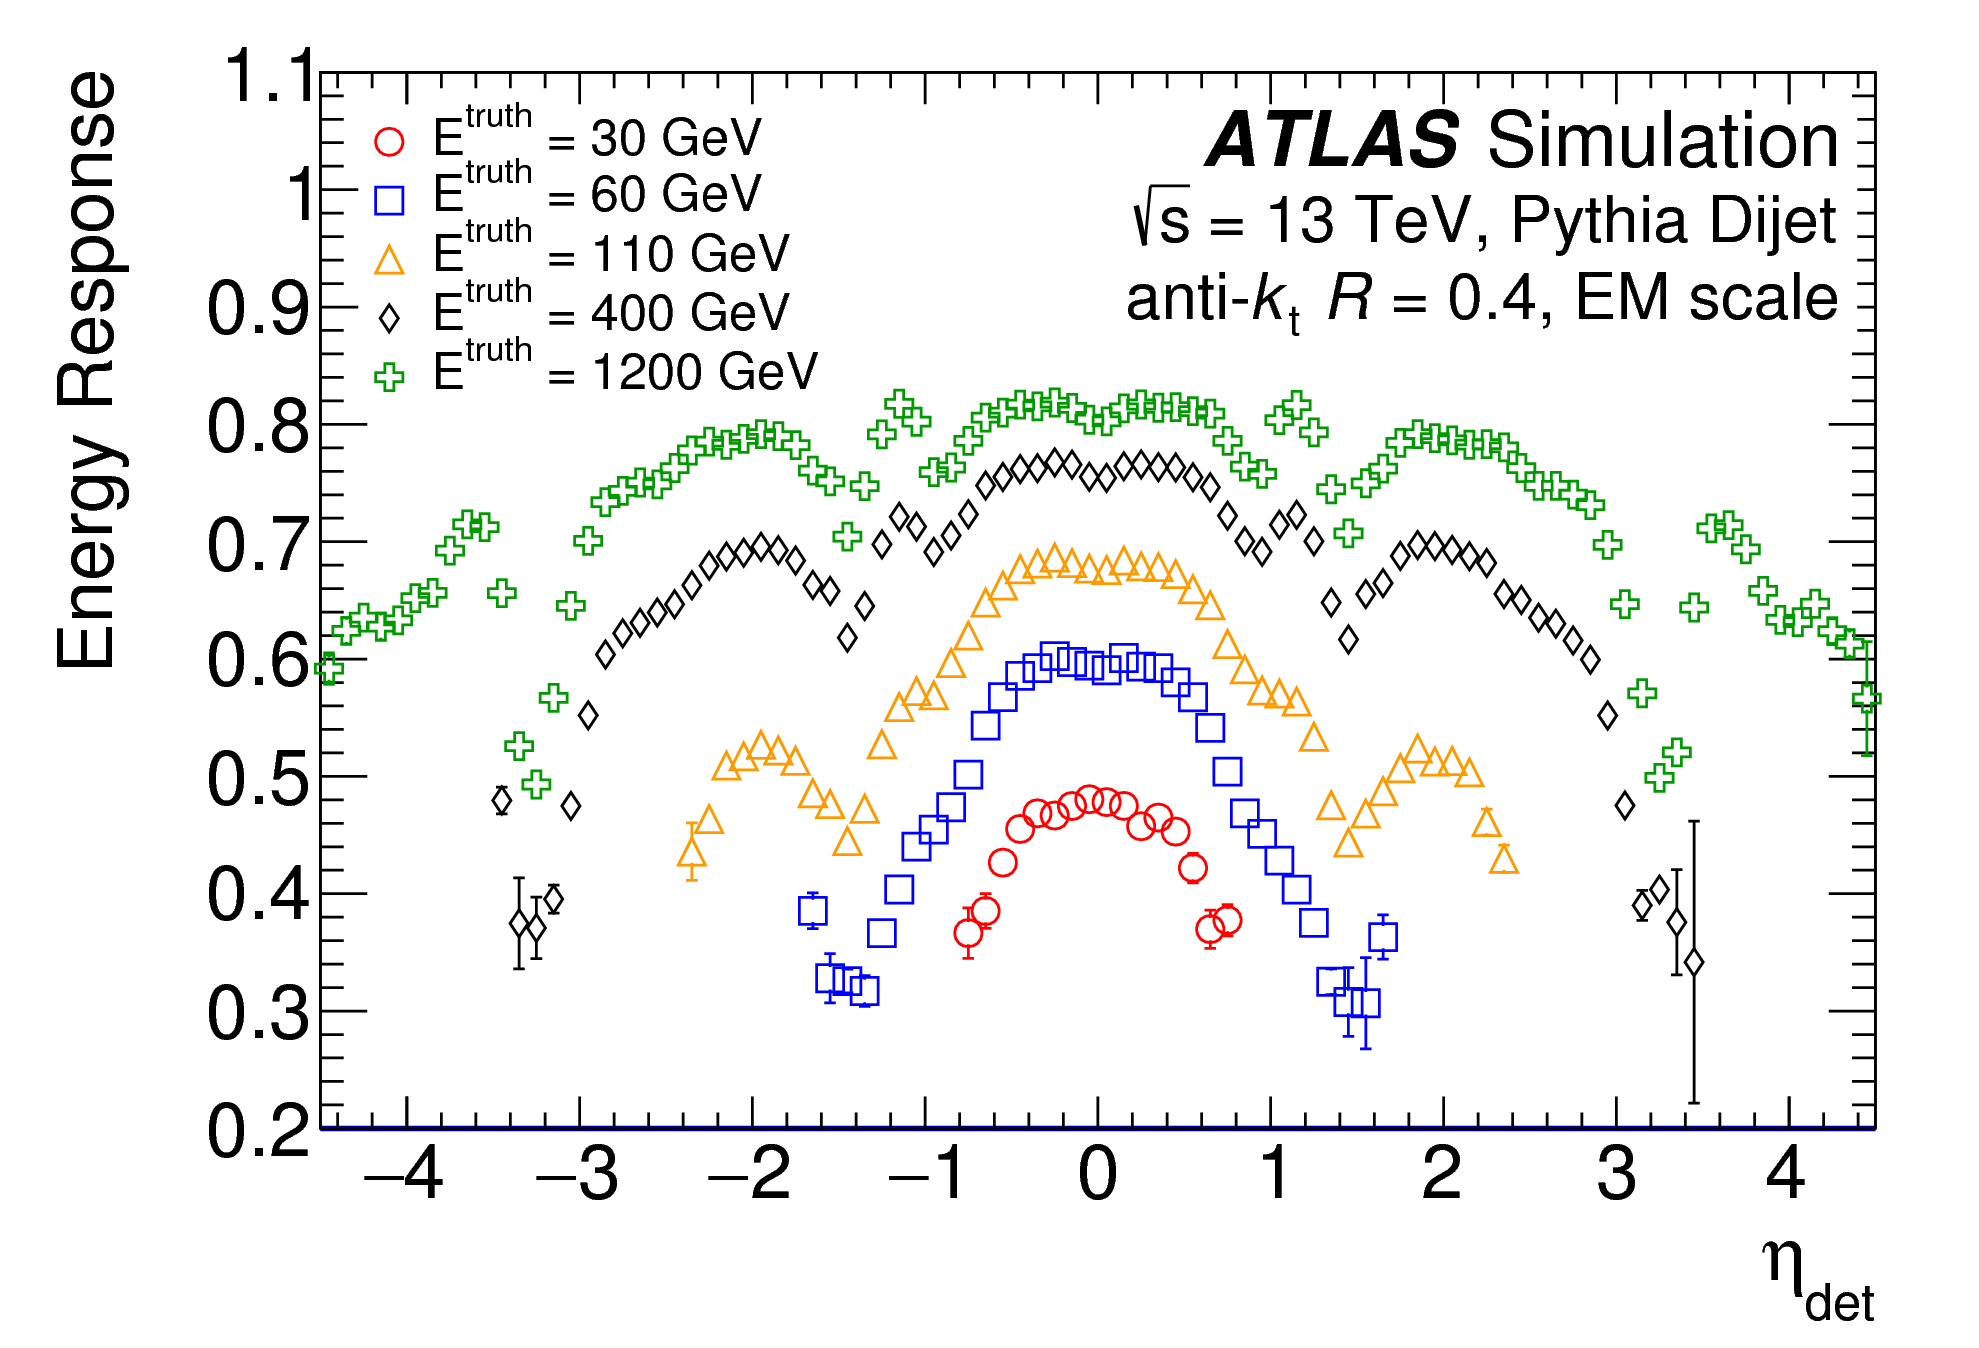
\includegraphics[width=0.48\textwidth]{figures/chapter3/jets/abs_jes_response}
        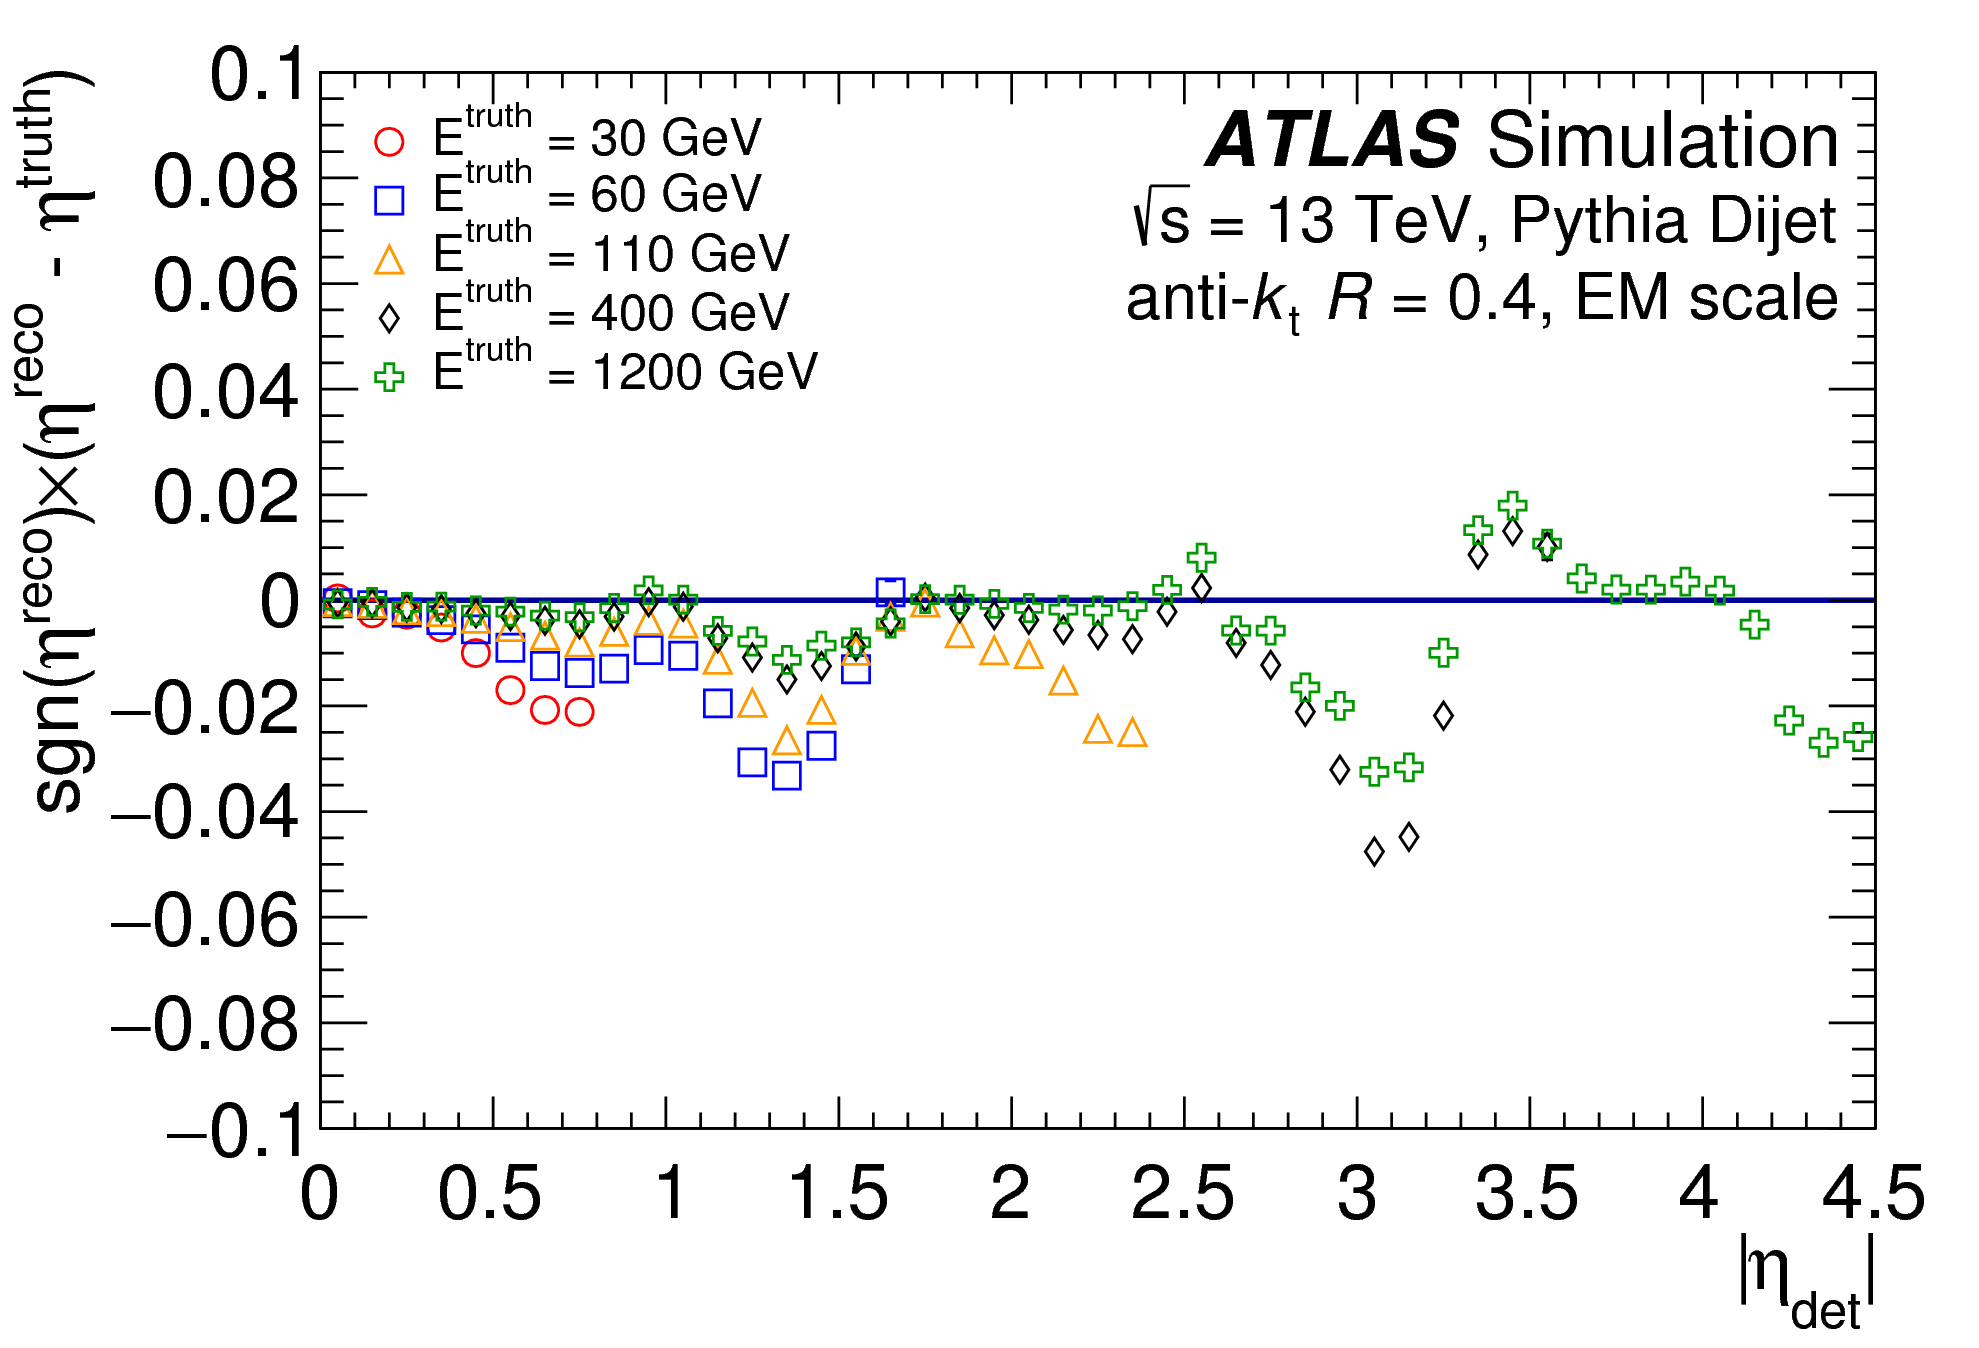
\includegraphics[width=0.48\textwidth]{figures/chapter3/jets/abs_jes_eta}
        \caption{
            \textit{Left}: Average energy response as a function of jet detector $\eta$, $\eta_{\text{det}}$.
            The colors correspond to different energy regimes for the particle-level jet to which the EM-scale
            reconstructed jet is matched. The inverse of the response is the final correction and can be seen to be
            largest for lower-\pT~jets.
            \textit{Right}: Difference in $\eta$ for the EM-scale reconstructed jet and the particle-level jet to which
            it is matched. The bias is clearly seen, with values typically negative, and it being largest
            for $\lvert \eta_{\text{det}} \rvert \sim 1.4$ $(\sim 3.1)$, corresponding to the barrel-endcap (endcap-forward)
            transition regions.
        }
        \label{fig:abs_jes_response}
    \end{center}
\end{figure}
\FloatBarrier

\subsubsection{Global Sequential Calibration}
\label{sec:jet_gsc}

The so-called Global Sequential Calibration (GSC) is a catch-all correction to account for remaining dependencies
of the EM-scale reconstructed jets on the jet shower shapes as well as fluctuations in the jet flavor composition and inter-jet energy distribution.
This correction improves the handling of fluctuations in the composition of the particles that initiate the jet; for example, correcting for the differences expected between quark- and gluon-initiated jets.
The former (quark-initiated) jets are typically more collimated with fewer, but higher-\pT, hadronic constituents.
The latter (gluon-initiated) jets typically contain many more, softer-\pT, particles and have wider transverse profiles
(and therefore do not traverse as far into the calorimeter).
The GSC has five stages, each following a numerical inversion of a corresponding jet response as in the case(s)
described in Section~\ref{sec:jet_eta_corr}, but are based on observables sensitive to the jet shower profile and growth
within the calorimeter as well as on the number and type of tracks associated with the reconstructed jet.
The use of tracking information from muons in this correction additionally helps with correcting the energy response of jets that
are not fully contained in the calorimeter, so-called \textit{punch-through jets}, but leak into the MS.

\subsubsection{In-situ Corrections}
\label{sec:jet_in_situ}

This last stage of the JES correction accounts for differences in jet response between data and simulation.
%The corrections derived here are applied to data, as opposed to the MC simulated jets as in the case of all previous
%corrections discussed up until this point.



%%%%%%%%%%%%%%%%%%%%%%%%%%%%%%%%%%%%%%%%%%%%%%%%%%%%%%%%%%%%%%%%%%%
%%%%%%%%%%%%%%%%%%%%%%%%%%%%%%%%%%%%%%%%%%%%%%%%%%%%%%%%%%%%%%%%%%%
% FLAVOR TAGGING
%%%%%%%%%%%%%%%%%%%%%%%%%%%%%%%%%%%%%%%%%%%%%%%%%%%%%%%%%%%%%%%%%%%
%%%%%%%%%%%%%%%%%%%%%%%%%%%%%%%%%%%%%%%%%%%%%%%%%%%%%%%%%%%%%%%%%%%
\section{Flavor Tagging of Jets}
\label{sec:flavor_tagging}

As in Ref.~\cite{ATL-PHYS-PUB-2017-013}.

\begin{figure}[!htb]
    \begin{center}
        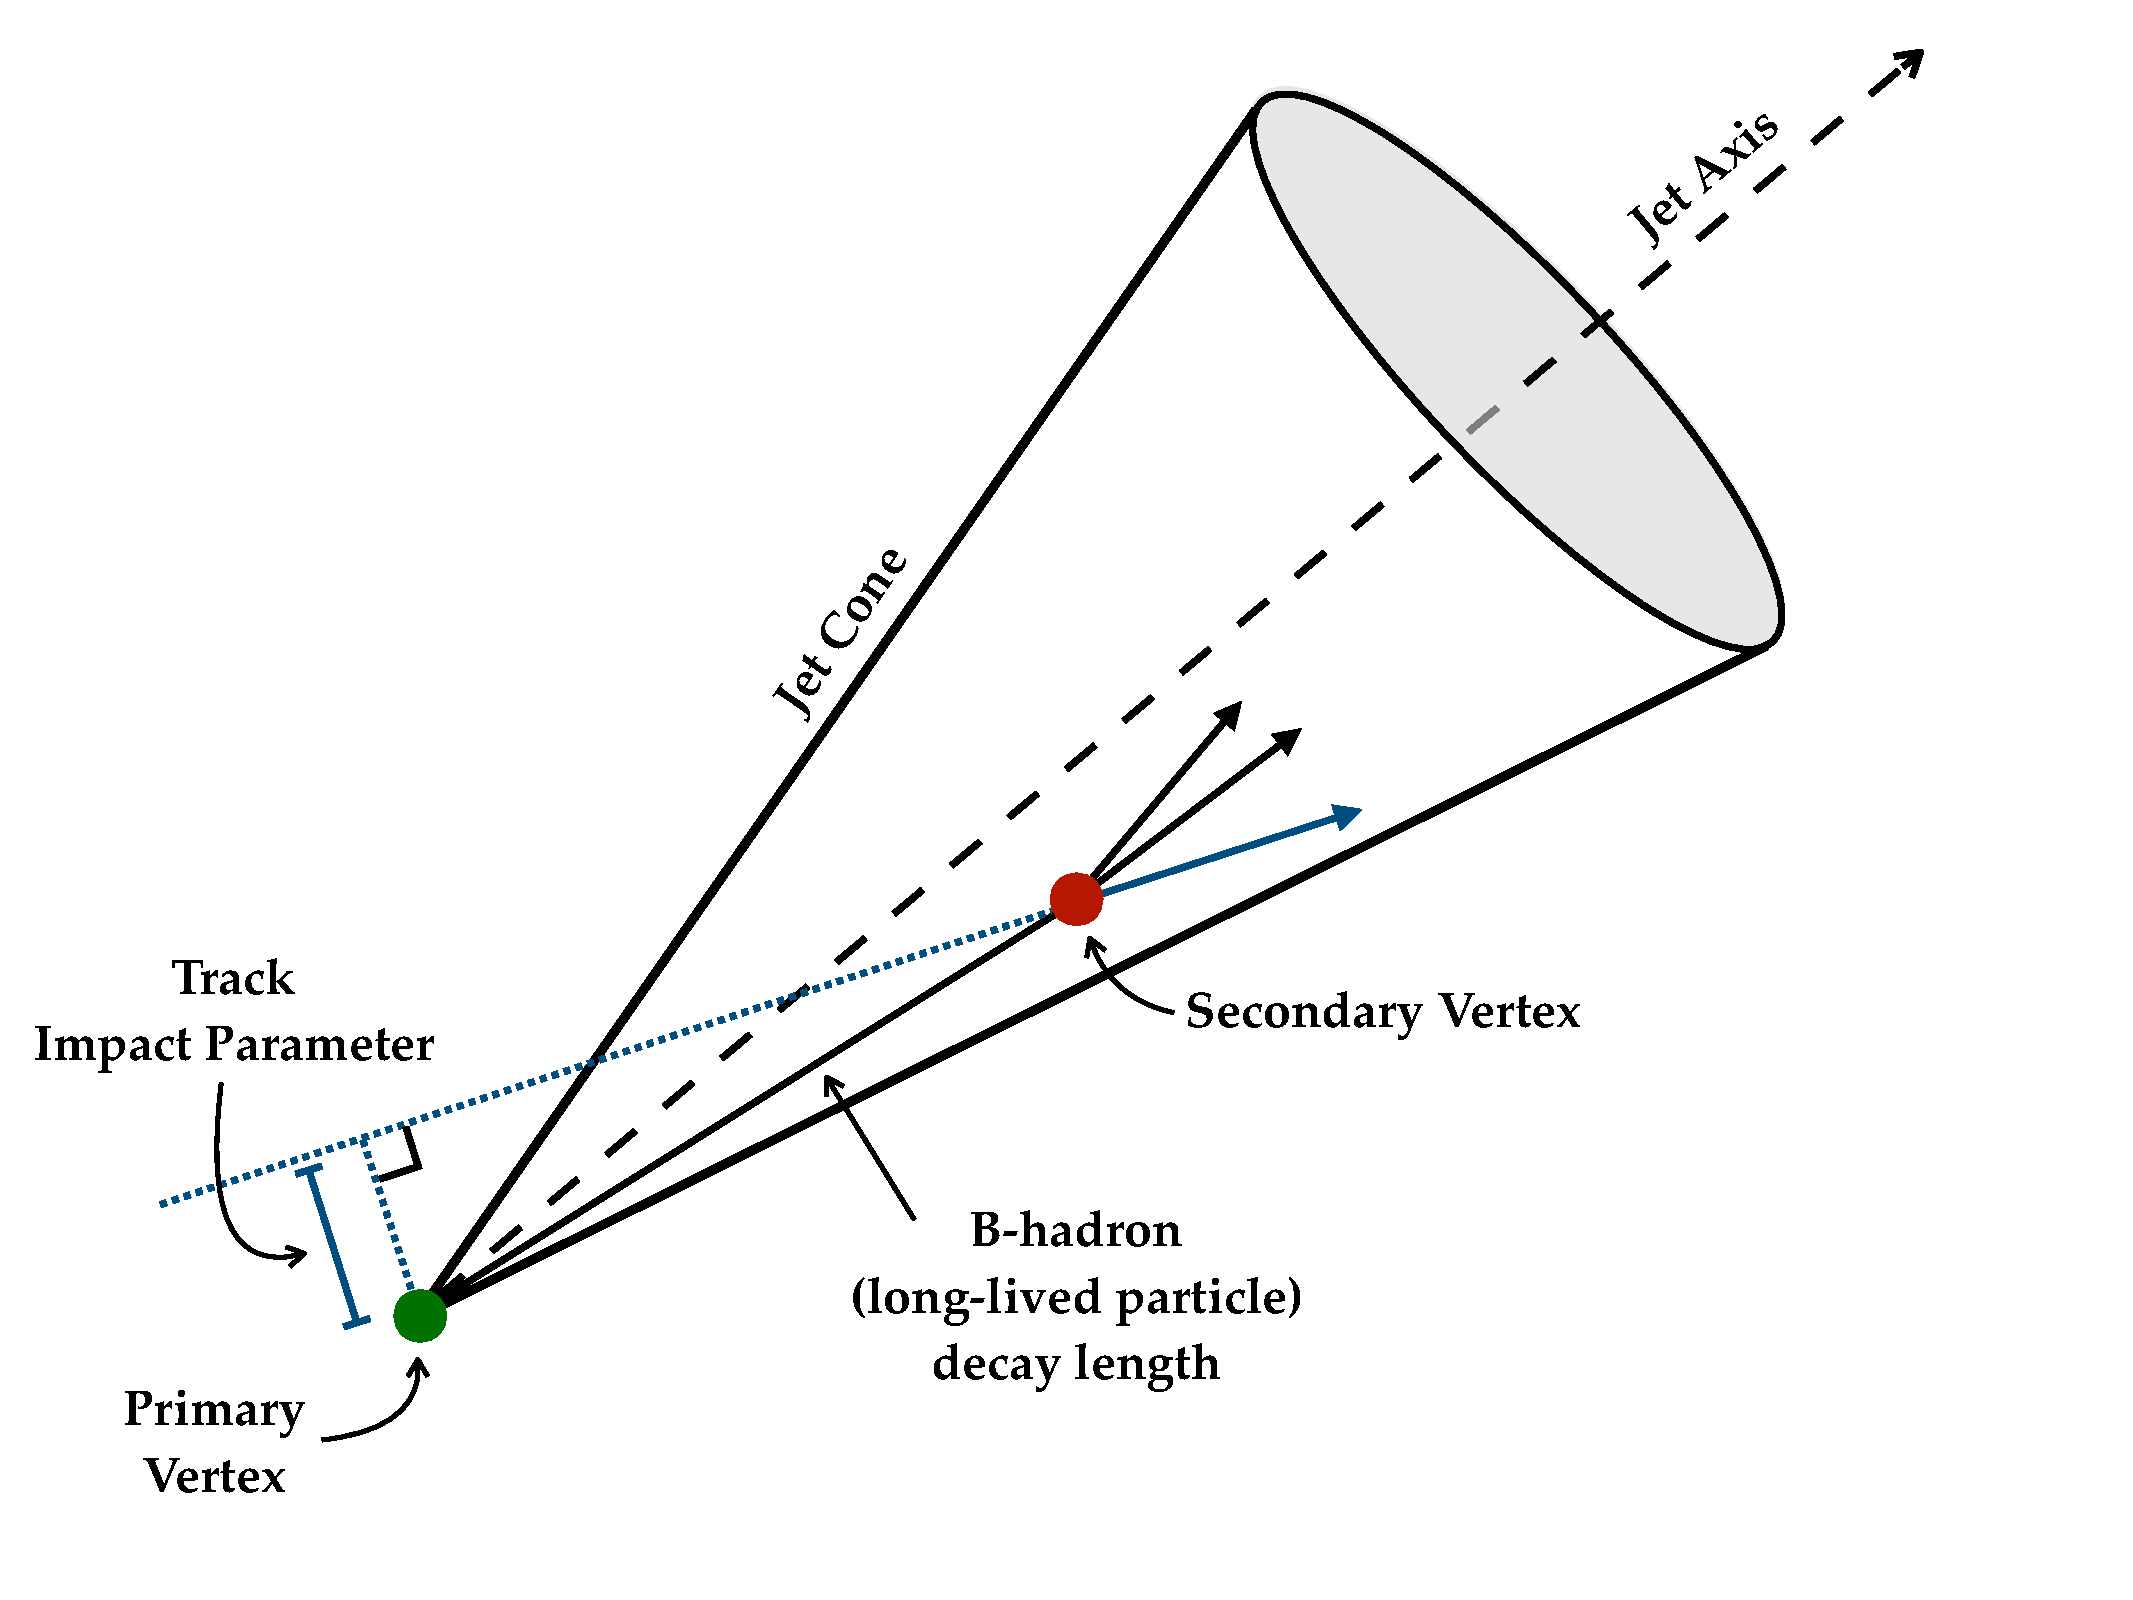
\includegraphics[width=0.7\textwidth]{figures/chapter3/ftag/bhadron_decayPDF}
        \caption{
        }
        \label{fig:bjet_decay}
    \end{center}
\end{figure}




\FloatBarrier


%%%%%%%%%%%%%%%%%%%%%%%%%%%%%%%%%%%%%%%%%%%%%%%%%%%%%%%%%%%%%%%%%%%
%%%%%%%%%%%%%%%%%%%%%%%%%%%%%%%%%%%%%%%%%%%%%%%%%%%%%%%%%%%%%%%%%%%
% MET
%%%%%%%%%%%%%%%%%%%%%%%%%%%%%%%%%%%%%%%%%%%%%%%%%%%%%%%%%%%%%%%%%%%
%%%%%%%%%%%%%%%%%%%%%%%%%%%%%%%%%%%%%%%%%%%%%%%%%%%%%%%%%%%%%%%%%%%
\section{The Missing Transverse Momentum}
\label{sec:met}


%%%%%%%%%%%%%%%%%%%%%%%%%%%%%%%%%%%%%%%%%%%%%%%%%%%%%%%%%%%%%%%%%%%
%%%%%%%%%%%%%%%%%%%%%%%%%%%%%%%%%%%%%%%%%%%%%%%%%%%%%%%%%%%%%%%%%%%
% MET
%%%%%%%%%%%%%%%%%%%%%%%%%%%%%%%%%%%%%%%%%%%%%%%%%%%%%%%%%%%%%%%%%%%
%%%%%%%%%%%%%%%%%%%%%%%%%%%%%%%%%%%%%%%%%%%%%%%%%%%%%%%%%%%%%%%%%%%
\section{Object-level Ambiguity Resolution}
\label{sec:object_ambiguity}


%\section{Ambiguity Solving}
